\documentclass[SE,lsstdraft,STR,toc]{lsstdoc}
\usepackage{geometry}
\usepackage{longtable,booktabs}
\usepackage{enumitem}
\usepackage{arydshln}

\input meta.tex

\providecommand{\tightlist}{
  \setlength{\itemsep}{0pt}\setlength{\parskip}{0pt}}

\begin{document}

\def\milestoneName{Camera Hexapod Functional Re-Verification}
\def\milestoneId{LVV-P63}
\def\product{SIT-COM Integration}

\setDocCompact{true}

\title{ LVV-P63 Camera Hexapod Functional Re-Verification Test Plan and Report}
\setDocRef{\lsstDocType-\lsstDocNum}
\date{\vcsdate}
\setDocUpstreamLocation{\url{https://github.com/lsst/lsst-texmf/examples}}
\author{ Austin Roberts }

\input history_and_info.tex


\setDocAbstract{
This is the test plan and report for LVV-P63 (Camera Hexapod Functional Re-Verification),
an LSST milestone pertaining to the System Engineering Subsystem.
}


\maketitle

\section{Introduction}
\label{sect:intro}


\subsection{Objectives}
\label{sect:objectives}

The objective of this test plan is to re-verify the functional
requirements of the Camera Hexapod's hardware and software, after
shipment from the vendors facility to the Summit, as defined in \citeds{LTS-206}
and \citeds{LTS-160}. This test campaign will only exercise the functionality
that was executed previously and meets the following criteria:

\begin{itemize}
\tightlist
\item
  Only requires the vendors EUI software and hardware via local control
\item
  Only requires a laser tracker
\item
  Does \textbf{NOT} require the camera rotator to be loaded with the
  camera simulated mass or actual camera hardware
\end{itemize}

The hardware functional requirements were previously verified during the
test campaign by the vendor at the vendors facility and accepted by LSST
during the Factory Acceptance Test review.



\subsection{System Overview}
\label{sect:systemoverview}

The Camera Hexapod is mounted to the Camera Rotator with the primary
function of aligning the camera with the optical path of the telescope.


\subsection{Document Overview}
\label{sect:docoverview}

This document was generated from Jira, obtaining the relevant information from the 
\href{https://jira.lsstcorp.org/secure/Tests.jspa#/testPlan/LVV-P63}{LVV-P63}
~Jira Test Plan and related Test Cycles (
  \href{https://jira.lsstcorp.org/secure/Tests.jspa#/testCycle/LVV-C114}{LVV-C114}
).

Section \ref{sect:intro} provides an overview of the test campaign, the system under test (\product{}), the applicable documentation, and explains how this document is organized.
Section \ref{sect:configuration}  describes the configuration used for this test.
Section \ref{sect:personnel} describes the necessary roles and lists the individuals assigned to them.
%Section \ref{sect:plannedtestactivities} provides the list of planned test cycles and test cases, including all relevant information that fully describes the test campaign.

Section \ref{sect:overview} provides a summary of the test results, including an overview in Table \ref{table:summary}, an overall assessment statement and suggestions for possible improvements.
Section \ref{sect:detailedtestresults} provides detailed results for each step in each test case.

The current status of test plan LVV-P63 in Jira is \textbf{ Draft }.

\subsection{References}
\label{sect:references}
\renewcommand{\refname}{}
\bibliography{lsst,refs,books,refs_ads,local}
\section{Test Configuration}
\label{sect:configuration}

\subsection{Data Collection}

  Observing is not required for this test campaign.

\subsection{Verification Environment}
\label{sect:hwconf}
  The Camera Hexapod will be verified in a climate controlled environment
on the 3rd floor of the Summit Facility integrated with the Camera Cable
Wrap on the Camera Cart.


  \subsection{Entry Criteria}
  In order to test the Camera Hexapod functionality, the following
criteria must be met first:

\begin{itemize}
\tightlist
\item
  All the test setup for the Data Acquisition system must be completed
  and ready to record data for the laser tracker and current probes
\item
  The Laser tracker and SMR's are installed and setup
\item
  The Inductive current probes are installed and setup
\item
  All utilities and electrical connections are hooked up and allow the
  Camera Hexapod to be powered on and controlled
\item
  The EFD must be set up to be able to store events and telemetry data
\end{itemize}


  \subsection{Exit Criteria}
  In order for this event to be considered complete, the following
criteria must be met:

\begin{itemize}
\tightlist
\item
  Raw test data, events, and telemetry have been saved for the Camera
  Hexapod.
\item
  All test data has been analyzed and post processed.
\item
  All test steps have been statused in the Jira Test Cases within this
  Test Plan and actual results populated as required.
\item
  A summary of the results of the test campaign has been captured in the
  Overall Assessment and Recommended Improvements fields of this Test
  Plan
\item
  A link to the verification artifacts used to produce the summary of
  results has been populated in the Verification Artifacts field of this
  Test Plan
\item
  Any failures have been captured in the
  \href{https://jira.lsstcorp.org/projects/FRACAS/issues/}{FRACAS}
  project
\end{itemize}


  \subsection{PMCS Activity}
  See Epics in Traceability Tab


\newpage
\section{Personnel}
\label{sect:personnel}

The personnel involved in the test campaign is shown in the following table.

\begin{longtable}{p{3cm}p{3cm}p{3cm}p{6cm}}
\hline
\multicolumn{2}{r}{Test Plan (LVV-P63) owner:} &
\multicolumn{2}{l}{\textbf{ Austin Roberts } }\\\hline
\multicolumn{2}{r}{ LVV-C114 owner:} &
\multicolumn{2}{l}{\textbf{
    Undefined
}
} \\\hline
\textbf{Test Case} & \textbf{Assigned to} & \textbf{Executed by} & \textbf{Additional Test Personnel} \\ \hline
\href{https://jira.lsstcorp.org/secure/Tests.jspa#/testCase/LVV-T1598}{LVV-T1598}
& {\small Kevin Siruno } & {\small  } &
\begin{minipage}[]{6cm}
\smallskip
{\small  }
\medskip
\end{minipage}
\\ \hline
\href{https://jira.lsstcorp.org/secure/Tests.jspa#/testCase/LVV-T1599}{LVV-T1599}
& {\small Kevin Siruno } & {\small  } &
\begin{minipage}[]{6cm}
\smallskip
{\small (1) Software Engineer\\
(1) Hardware Engineer
 }
\medskip
\end{minipage}
\\ \hline
\href{https://jira.lsstcorp.org/secure/Tests.jspa#/testCase/LVV-T1600}{LVV-T1600}
& {\small Kevin Siruno } & {\small  } &
\begin{minipage}[]{6cm}
\smallskip
{\small (1) Software Engineer\\
(1) Hardware Engineer
 }
\medskip
\end{minipage}
\\ \hline
\end{longtable}

\newpage

\section{Test Campaign Overview}
\label{sect:overview}

\subsection{Summary}
\label{sect:summarytable}

\begin{longtable}{p{2cm}p{2.5cm}p{9cm}p{2.5cm}}
\toprule
\multicolumn{3}{l}{ Test Plan {\bf LVV-P63: Camera Hexapod Functional Re-verification
 }} & Draft \\\hline

  \multicolumn{3}{l}{ Test Cycle {\bf LVV-C114: Camera Hexapod Re-verification
 }} & Not Executed \\\hline

  {\bf \footnotesize test case} & {\bf \footnotesize status} & {\bf \footnotesize comment} & {\bf \footnotesize issues} \\\toprule

    \href{https://jira.lsstcorp.org/secure/Tests.jspa#/testCase/LVV-T1598}{LVV-T1598}
    & Not Executed &
    \begin{minipage}[]{9cm}
    \smallskip
    
    \medskip
    \end{minipage}
    &
    \\\hline
    \href{https://jira.lsstcorp.org/secure/Tests.jspa#/testCase/LVV-T1599}{LVV-T1599}
    & Not Executed &
    \begin{minipage}[]{9cm}
    \smallskip
    
    \medskip
    \end{minipage}
    &
    \\\hline
    \href{https://jira.lsstcorp.org/secure/Tests.jspa#/testCase/LVV-T1600}{LVV-T1600}
    & Not Executed &
    \begin{minipage}[]{9cm}
    \smallskip
    
    \medskip
    \end{minipage}
    &
    \\\hline
\caption{Test Results Summary}
\label{table:summary}
\end{longtable}

\subsection{Overall Assessment}
\label{sect:overallassessment}

Not yet available.

\subsection{Recommended Improvements}
\label{sect:recommendations}

Not yet available.

\newpage
\section{Detailed Test Results}
\label{sect:detailedtestresults}

\subsection{Test Cycle LVV-C114 }

Open test cycle {\it \href{https://jira.lsstcorp.org/secure/Tests.jspa#/testrun/LVV-C114}{Camera Hexapod Re-verification
}} in Jira.

Camera Hexapod Re-verification
\\
Status: Not Executed



\subsubsection{Software Version/Baseline}
Not provided.

\subsubsection{Configuration}
Not provided.

\subsubsection{Test Cases in LVV-C114 Test Cycle}

\paragraph{Test Case LVV-T1598 - Camera Hexapod Hardware Functional Re-verification
 }\mbox{}\\

Open  \href{https://jira.lsstcorp.org/secure/Tests.jspa#/testCase/LVV-T1598}{\textit{ LVV-T1598 } }
test case in Jira.

The objective of this test case is to re-verify the functional
requirements of the camera hexapod's hardware, after shipment from the
vendors facility to the Summit, as defined in \citeds{LTS-206}. This test case
will only exercise the functionality that was executed previously and
meets the following criteria:

\begin{itemize}
\tightlist
\item
  Only requires the camera hexapod to be operable {\textbf{This is
  assuming we don't need the rotator turned on for anything which seems
  unlikely}}
\item
  Only requires the vendors EUI software and hardware via local control
\item
  Only requires a laser tracker
\item
  Does \textbf{NOT} require the camera rotator to be loaded with the
  camera simulated mass or actual camera hardware
\end{itemize}

The hardware functional requirements were previously verified during the
test campaign by the vendor at the vendors facility and accepted by LSST
during the Factory Acceptance Test review. The test procedure used
during the vendor's acceptance testing is the \emph{LSST
Hexapods-Rotator Acceptance Test Procedure} which is attached to this
test case. The test steps of this test case reference that document for
the details on how to perform the test in a similar way as was performed
previously and includes deviations to that document due to the
differences in the verification configuration and deviations to
requirements granted to the vendor by LSST.\\[2\baselineskip]See the
attached \emph{LSST Rotator Hexapod's Manual} for more information on
how to operate the hexapod.


\textbf{ Preconditions}:\\
Prior to the execution of this test case to re-verify the Camera Hexapod
hardware functional requirements, the following Summit tasks must be
completed:

\begin{itemize}
\tightlist
\item
  The Hexapod has been installed on the camera cart

  \begin{itemize}
  \tightlist
  \item
    \url{https://jira.lsstcorp.org/browse/SUMMIT-3224}
  \end{itemize}
\item
  The Hexapod Controller has been deployed on the summit

  \begin{itemize}
  \tightlist
  \item
    \url{https://jira.lsstcorp.org/browse/SUMMIT-3229}
  \end{itemize}
\item
  Boxes for the Hexapod have been transported to the 3rd level

  \begin{itemize}
  \tightlist
  \item
    \url{https://jira.lsstcorp.org/browse/SUMMIT-3230}
  \end{itemize}
\item
  All Hexapod cables and cabinets have been prepared for integration
  with camera cart

  \begin{itemize}
  \tightlist
  \item
    \url{https://jira.lsstcorp.org/browse/SUMMIT-3231}
  \end{itemize}
\item
  The offset has been installed onto the integrating structure

  \begin{itemize}
  \tightlist
  \item
    \url{https://jira.lsstcorp.org/browse/SUMMIT-3293}
  \end{itemize}
\item
  The Camera Hexapod electrical connections have been tested

  \begin{itemize}
  \tightlist
  \item
    \url{https://jira.lsstcorp.org/browse/SUMMIT-3294}
  \end{itemize}
\end{itemize}


Execution status: {\bf Not Executed }

Final comment:\\


Detailed steps results:

\begin{longtable}{p{1cm}p{15cm}}
\hline
{Step} & Step Details\\ \hline
1 & Description \\
 & \begin{minipage}[t]{15cm}
{\footnotesize
\smallskip
\textbf{STARTING THE EUI}\\[2\baselineskip]Double click the Hexapod GUI
Viewer desktop icon on the computer.

\begin{itemize}
\tightlist
\item
  This can be done on the Dell Management PC or another computer on the
  same network
\end{itemize}

\medskip }
\end{minipage}
\\ \cdashline{2-2}


 & Expected Result \\
 & \begin{minipage}[t]{15cm}{\footnotesize
\smallskip
A prompt to enter the password is shown.

\medskip }
\end{minipage} \\ \cdashline{2-2}

 & Actual Result \\
 & \begin{minipage}[t]{15cm}{\footnotesize
\smallskip

\medskip }
\end{minipage} \\ \cdashline{2-2}

 & Status: \textbf{ Not Executed } \\ \hline

2 & Description \\
 & \begin{minipage}[t]{15cm}
{\footnotesize
\smallskip
Enter the password ``lsst-vnc''

\begin{itemize}
\tightlist
\item
  If the EUI isn't automatically up and running when the VNC opens,
  double click on the Hexapod-eGUI icon on the VNC viewer
\end{itemize}

\medskip }
\end{minipage}
\\ \cdashline{2-2}


 & Expected Result \\
 & \begin{minipage}[t]{15cm}{\footnotesize
\smallskip
The EUI is in the Offline State/PublishOnly substate and is able to
publish through SAL but cannot receive commands.

\medskip }
\end{minipage} \\ \cdashline{2-2}

 & Actual Result \\
 & \begin{minipage}[t]{15cm}{\footnotesize
\smallskip

\medskip }
\end{minipage} \\ \cdashline{2-2}

 & Status: \textbf{ Not Executed } \\ \hline

3 & Description \\
 & \begin{minipage}[t]{15cm}
{\footnotesize
\smallskip
\textbf{OFFLINESTATE/AVAILABLESTATE}\\
On the Main tab, select the ``Offline SubState Cmd'' field in the
Commands to Send section, set the Offline SubState Triggers to ``System
Ready'' and click on the Send Command button.\\
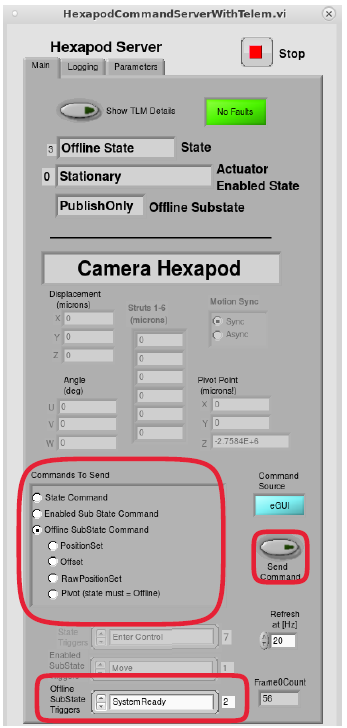
\includegraphics[width=1.79167in]{jira_imgs/1024.png}

\medskip }
\end{minipage}
\\ \cdashline{2-2}


 & Expected Result \\
 & \begin{minipage}[t]{15cm}{\footnotesize
\smallskip
The system transitions from the OfflineState/PublishOnly substate to the
OfflineState/AvailableState substate and the Command Source says
eGUI.\\[2\baselineskip]

\medskip }
\end{minipage} \\ \cdashline{2-2}

 & Actual Result \\
 & \begin{minipage}[t]{15cm}{\footnotesize
\smallskip

\medskip }
\end{minipage} \\ \cdashline{2-2}

 & Status: \textbf{ Not Executed } \\ \hline

4 & Description \\
 & \begin{minipage}[t]{15cm}
{\footnotesize
\smallskip
\textbf{OFFLINESTATE -\textgreater{} STANDBYSTATE}\\
Click on the State Command field in the Commands to Send section.\\
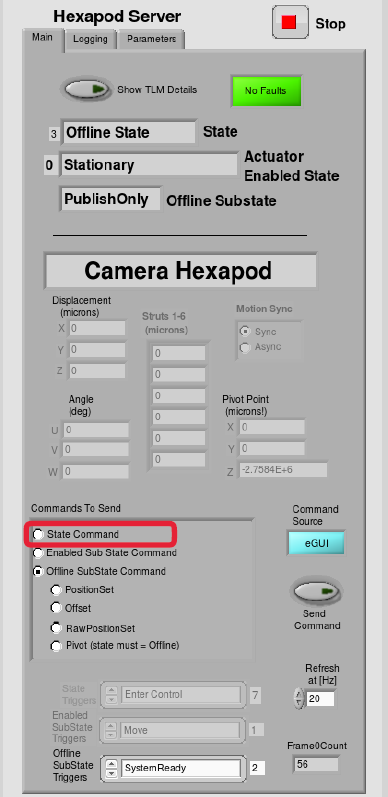
\includegraphics[width=1.79167in]{jira_imgs/1028.png}

\medskip }
\end{minipage}
\\ \cdashline{2-2}


 & Expected Result \\
 & \begin{minipage}[t]{15cm}{\footnotesize
\smallskip
The State Triggers dialogue box shown below becomes visible.\\
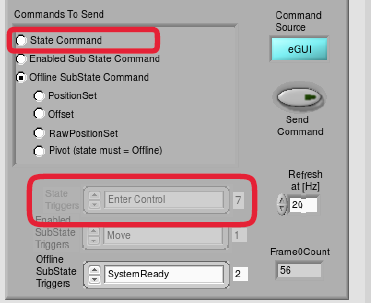
\includegraphics[width=1.79167in]{jira_imgs/1029.png}

\medskip }
\end{minipage} \\ \cdashline{2-2}

 & Actual Result \\
 & \begin{minipage}[t]{15cm}{\footnotesize
\smallskip

\medskip }
\end{minipage} \\ \cdashline{2-2}

 & Status: \textbf{ Not Executed } \\ \hline

5 & Description \\
 & \begin{minipage}[t]{15cm}
{\footnotesize
\smallskip
Scroll through the available trigger options to select ``Enter Control''
and click the Send Command button.

\medskip }
\end{minipage}
\\ \cdashline{2-2}


 & Expected Result \\
 & \begin{minipage}[t]{15cm}{\footnotesize
\smallskip
The system transitions to the Standby state and the primary state
display box at the top of the Main says Standby State.

\medskip }
\end{minipage} \\ \cdashline{2-2}

 & Actual Result \\
 & \begin{minipage}[t]{15cm}{\footnotesize
\smallskip

\medskip }
\end{minipage} \\ \cdashline{2-2}

 & Status: \textbf{ Not Executed } \\ \hline

6 & Description \\
 & \begin{minipage}[t]{15cm}
{\footnotesize
\smallskip
\textbf{STANDBYSTATE -\textgreater{} DISABLEDSTATE}\\
From the StandbyState, send a Start State command.

\medskip }
\end{minipage}
\\ \cdashline{2-2}


 & Expected Result \\
 & \begin{minipage}[t]{15cm}{\footnotesize
\smallskip
The system transitions into DisabledState and the current configuration
parameters are maintained from the default parameters or from the
previous DDS start command.~

\medskip }
\end{minipage} \\ \cdashline{2-2}

 & Actual Result \\
 & \begin{minipage}[t]{15cm}{\footnotesize
\smallskip

\medskip }
\end{minipage} \\ \cdashline{2-2}

 & Status: \textbf{ Not Executed } \\ \hline

7 & Description \\
 & \begin{minipage}[t]{15cm}
{\footnotesize
\smallskip
\textbf{DISABLEDSTATE -\textgreater{} ENABLEDSTATE}\\
From the DisabledState, send an Enable State Command.~

\medskip }
\end{minipage}
\\ \cdashline{2-2}


 & Expected Result \\
 & \begin{minipage}[t]{15cm}{\footnotesize
\smallskip
The system transitions into the EnabledState/Stationary substate, the
motor drives are enabled and and motion can be commanded.~

\medskip }
\end{minipage} \\ \cdashline{2-2}

 & Actual Result \\
 & \begin{minipage}[t]{15cm}{\footnotesize
\smallskip

\medskip }
\end{minipage} \\ \cdashline{2-2}

 & Status: \textbf{ Not Executed } \\ \hline

8 & Description \\
 & \begin{minipage}[t]{15cm}
{\footnotesize
\smallskip
\textless{}conditional state\textgreater{}\\
\textbf{FAULTSTATE}\\
If a Fault occurs in any of the other states, the system will
automatically transition to the Fault State. While in the Fault state,
send a clearError.\\
Note: If the fault that occurs goes through the interlock system, reset
the safety relay switch and send a clearError command.

\medskip }
\end{minipage}
\\ \cdashline{2-2}


 & Expected Result \\
 & \begin{minipage}[t]{15cm}{\footnotesize
\smallskip
The system transitions back to the OfflineState/PublishOnly substate.
(Go back to Step 3)

\medskip }
\end{minipage} \\ \cdashline{2-2}

 & Actual Result \\
 & \begin{minipage}[t]{15cm}{\footnotesize
\smallskip

\medskip }
\end{minipage} \\ \cdashline{2-2}

 & Status: \textbf{ Not Executed } \\ \hline

9 & Description \\
 & \begin{minipage}[t]{15cm}
{\footnotesize
\smallskip
\textbf{Follow \emph{3.3.1 Positioning} of the LSST Hexapods-Rotator
Acceptance Test Procedure, Sheet 23-24.}

\medskip }
\end{minipage}
\\ \cdashline{2-2}

 & Test Data \\
 & \begin{minipage}[t]{15cm}{\footnotesize
\smallskip
\textbf{Deviation:~}Test this with no performance payload and at a
single elevation angle of zero degrees.

\medskip }
\end{minipage} \\ \cdashline{2-2}

 & Expected Result \\
 & \begin{minipage}[t]{15cm}{\footnotesize
\smallskip
The position of the hexapod is able to be commanded and no software
limits or limit switches are tripped.

\medskip }
\end{minipage} \\ \cdashline{2-2}

 & Actual Result \\
 & \begin{minipage}[t]{15cm}{\footnotesize
\smallskip

\medskip }
\end{minipage} \\ \cdashline{2-2}

 & Status: \textbf{ Not Executed } \\ \hline

10 & Description \\
 & \begin{minipage}[t]{15cm}
{\footnotesize
\smallskip
\textbf{Follow \emph{3.3.2 Centers of Rotation} of the LSST
Hexapods-Rotator Acceptance Test Procedure, Sheet 24-25.}

\medskip }
\end{minipage}
\\ \cdashline{2-2}

 & Test Data \\
 & \begin{minipage}[t]{15cm}{\footnotesize
\smallskip
\textbf{Deviation:~}Record pivot position through the EUI.

\medskip }
\end{minipage} \\ \cdashline{2-2}

 & Expected Result \\
 & \begin{minipage}[t]{15cm}{\footnotesize
\smallskip
The center of rotation is able to be moved.

\medskip }
\end{minipage} \\ \cdashline{2-2}

 & Actual Result \\
 & \begin{minipage}[t]{15cm}{\footnotesize
\smallskip

\medskip }
\end{minipage} \\ \cdashline{2-2}

 & Status: \textbf{ Not Executed } \\ \hline

11 & Description \\
 & \begin{minipage}[t]{15cm}
{\footnotesize
\smallskip
\textbf{Follow \emph{3.3.3 Cross-Talk Motion~}of the LSST
Hexapods-Rotator Acceptance Test Procedure, Sheet 25.}

\medskip }
\end{minipage}
\\ \cdashline{2-2}


 & Expected Result \\
 & \begin{minipage}[t]{15cm}{\footnotesize
\smallskip
There is no cross-talk observed (actuator positioning errors and
erroneous geometry are minimal)

\medskip }
\end{minipage} \\ \cdashline{2-2}

 & Actual Result \\
 & \begin{minipage}[t]{15cm}{\footnotesize
\smallskip

\medskip }
\end{minipage} \\ \cdashline{2-2}

 & Status: \textbf{ Not Executed } \\ \hline

12 & Description \\
 & \begin{minipage}[t]{15cm}
{\footnotesize
\smallskip
\textbf{Follow \emph{3.3.4 Radial (X and Y) Translational Range~}of the
LSST Hexapods-Rotator Acceptance Test Procedure, Sheet 25.}

\medskip }
\end{minipage}
\\ \cdashline{2-2}

 & Test Data \\
 & \begin{minipage}[t]{15cm}{\footnotesize
\smallskip
\textbf{Deviation:~}Only test at a zero degree elevation angle.

\medskip }
\end{minipage} \\ \cdashline{2-2}

 & Expected Result \\
 & \begin{minipage}[t]{15cm}{\footnotesize
\smallskip
The hexapod is capable of moving to the positions in the XY plane listed
in the Acceptance Test Procedure.

\medskip }
\end{minipage} \\ \cdashline{2-2}

 & Actual Result \\
 & \begin{minipage}[t]{15cm}{\footnotesize
\smallskip

\medskip }
\end{minipage} \\ \cdashline{2-2}

 & Status: \textbf{ Not Executed } \\ \hline

13 & Description \\
 & \begin{minipage}[t]{15cm}
{\footnotesize
\smallskip
\textbf{Follow \emph{3.3.6 Axial (Z) Translation Range~}of the LSST
Hexapods-Rotator Acceptance Test Procedure, Sheet 27.}

\medskip }
\end{minipage}
\\ \cdashline{2-2}

 & Test Data \\
 & \begin{minipage}[t]{15cm}{\footnotesize
\smallskip
\textbf{Deviation:~}Only test at a zero degree elevation angle.

\medskip }
\end{minipage} \\ \cdashline{2-2}

 & Expected Result \\
 & \begin{minipage}[t]{15cm}{\footnotesize
\smallskip
The hexapod is capable of moving to the positions in the Z plane listed
in the Acceptance Test Procedure.~

\medskip }
\end{minipage} \\ \cdashline{2-2}

 & Actual Result \\
 & \begin{minipage}[t]{15cm}{\footnotesize
\smallskip

\medskip }
\end{minipage} \\ \cdashline{2-2}

 & Status: \textbf{ Not Executed } \\ \hline

14 & Description \\
 & \begin{minipage}[t]{15cm}
{\footnotesize
\smallskip
\textbf{Follow \emph{3.3.8 Rotational Range Around X-Axis (Tip) and
Y-Axis (Tilt)~}of the LSST Hexapods-Rotator Acceptance Test Procedure,
Sheet 28-29.}

\medskip }
\end{minipage}
\\ \cdashline{2-2}

 & Test Data \\
 & \begin{minipage}[t]{15cm}{\footnotesize
\smallskip
\textbf{Deviation:~}Only test at a zero degree elevation angle.

\medskip }
\end{minipage} \\ \cdashline{2-2}

 & Expected Result \\
 & \begin{minipage}[t]{15cm}{\footnotesize
\smallskip
The hexapod is capable of moving to the positions in the RXRY plane
listed in the Acceptance Test Procedure.

\medskip }
\end{minipage} \\ \cdashline{2-2}

 & Actual Result \\
 & \begin{minipage}[t]{15cm}{\footnotesize
\smallskip

\medskip }
\end{minipage} \\ \cdashline{2-2}

 & Status: \textbf{ Not Executed } \\ \hline

15 & Description \\
 & \begin{minipage}[t]{15cm}
{\footnotesize
\smallskip
\textbf{Follow \emph{3.3.10 Rotation Range Around Z-Axis (Twist)~}of the
LSST Hexapods-Rotator Acceptance Test Procedure, Sheet 30.}

\medskip }
\end{minipage}
\\ \cdashline{2-2}

 & Test Data \\
 & \begin{minipage}[t]{15cm}{\footnotesize
\smallskip
\textbf{Deviation:~}Only test at a zero degree elevation angle.

\medskip }
\end{minipage} \\ \cdashline{2-2}

 & Expected Result \\
 & \begin{minipage}[t]{15cm}{\footnotesize
\smallskip
The hexapod is capable of moving to the positions in the RZ-axis listed
in the Acceptance Test Procedure.

\medskip }
\end{minipage} \\ \cdashline{2-2}

 & Actual Result \\
 & \begin{minipage}[t]{15cm}{\footnotesize
\smallskip

\medskip }
\end{minipage} \\ \cdashline{2-2}

 & Status: \textbf{ Not Executed } \\ \hline

16 & Description \\
 & \begin{minipage}[t]{15cm}
{\footnotesize
\smallskip
\textbf{Follow \emph{3.3.13 Hexapod Absolute Accuracy~}of the LSST
Hexapods-Rotator Acceptance Test Procedure, Sheet 38-42.}

\medskip }
\end{minipage}
\\ \cdashline{2-2}

 & Test Data \\
 & \begin{minipage}[t]{15cm}{\footnotesize
\smallskip
\textbf{Deviation:~}Only test at a zero degree elevation angle.

\medskip }
\end{minipage} \\ \cdashline{2-2}

 & Expected Result \\
 & \begin{minipage}[t]{15cm}{\footnotesize
\smallskip
The accuracy of the hexapod is good enough to be consistently repeated.

\medskip }
\end{minipage} \\ \cdashline{2-2}

 & Actual Result \\
 & \begin{minipage}[t]{15cm}{\footnotesize
\smallskip

\medskip }
\end{minipage} \\ \cdashline{2-2}

 & Status: \textbf{ Not Executed } \\ \hline

17 & Description \\
 & \begin{minipage}[t]{15cm}
{\footnotesize
\smallskip
\textbf{Follow \emph{3.3.16 Hexapod Radial (X and Y) and Axial (Z)
Velocity Range and~3.3.17 Hexapod Rotational Velocity~}of the LSST
Hexapods-Rotator Acceptance Test Procedure, Sheet 43-44.}

\medskip }
\end{minipage}
\\ \cdashline{2-2}

 & Test Data \\
 & \begin{minipage}[t]{15cm}{\footnotesize
\smallskip
\textbf{Deviation:~}Only test this using synchronous mode.

\medskip }
\end{minipage} \\ \cdashline{2-2}

 & Expected Result \\
 & \begin{minipage}[t]{15cm}{\footnotesize
\smallskip
The hexapod velocity exceeds the 152um/s in XY and 0.0039deg/s in RXYRY
and RZ requirements.

\medskip }
\end{minipage} \\ \cdashline{2-2}

 & Actual Result \\
 & \begin{minipage}[t]{15cm}{\footnotesize
\smallskip

\medskip }
\end{minipage} \\ \cdashline{2-2}

 & Status: \textbf{ Not Executed } \\ \hline

18 & Description \\
 & \begin{minipage}[t]{15cm}
{\footnotesize
\smallskip
\textbf{Follow \emph{3.3.18 Hexapod Heat Dissipation~}of the LSST
Hexapods-Rotator Acceptance Test Procedure, Sheet 44.}

\medskip }
\end{minipage}
\\ \cdashline{2-2}


 & Expected Result \\
 & \begin{minipage}[t]{15cm}{\footnotesize
\smallskip
The current measured by the inductive current probes is calculated to
meet the heat dissipation requirement.

\medskip }
\end{minipage} \\ \cdashline{2-2}

 & Actual Result \\
 & \begin{minipage}[t]{15cm}{\footnotesize
\smallskip

\medskip }
\end{minipage} \\ \cdashline{2-2}

 & Status: \textbf{ Not Executed } \\ \hline

\end{longtable}

\paragraph{Test Case LVV-T1599 - Camera Hexapod Software Functional Re-verification
 }\mbox{}\\

Open  \href{https://jira.lsstcorp.org/secure/Tests.jspa#/testCase/LVV-T1599}{\textit{ LVV-T1599 } }
test case in Jira.

The objective of this test case is to re-verify the functional
requirements of the camera hexapod's software, after shipment of the
hardware from the vendor's facility to the Summit, as defined in \citeds{LTS-206}
and \citeds{LTS-160}. This test case will only exercise the functionality that
was executed previously and meets the following criteria:

\begin{itemize}
\tightlist
\item
  Only requires the camera hexapod to be operable
\item
  Only requires testing of the synchronous mode

  \begin{itemize}
  \tightlist
  \item
    \textbf{Asynchronous mode is not a standard mode of operation}
  \end{itemize}
\item
  Only requires the vendors EUI software and hardware via local control

  \begin{itemize}
  \tightlist
  \item
    Does \textbf{NOT} require integration with SAL
  \end{itemize}
\item
  Does \textbf{NOT} require the camera hexapod to be loaded with the
  camera simulated mass or actual camera hardware
\end{itemize}

The software functional requirements were previously verified during the
test campaign by the vendor at the vendor's facility and accepted by
LSST during the Factory Acceptance Test review. The test procedure used
during the vendor's acceptance testing is the \emph{LSST
Hexapods-Rotator Software Acceptance Test Procedure} which is attached
to this test case. The test steps of this test case are taken directly
from that document on how to perform the test in a similar way as was
performed previously and includes changes noted by the
vendor.\\[2\baselineskip]See the attached \emph{LSST Rotator Hexapod's
Manual} for more information on how to operate the hexapod.


\textbf{ Preconditions}:\\
Prior to the execution of this test case to re-verify the Camera Hexapod
hardware functional requirements, the following Summit tasks must be
completed:

\begin{itemize}
\tightlist
\item
  The Hexapod has been installed on the camera cart

  \begin{itemize}
  \tightlist
  \item
    \url{https://jira.lsstcorp.org/browse/SUMMIT-3224}
  \end{itemize}
\item
  The Hexapod Controller has been deployed on the summit

  \begin{itemize}
  \tightlist
  \item
    \url{https://jira.lsstcorp.org/browse/SUMMIT-3229}
  \end{itemize}
\item
  Boxes for the Hexapod have been transported to the 3rd level

  \begin{itemize}
  \tightlist
  \item
    \url{https://jira.lsstcorp.org/browse/SUMMIT-3230}
  \end{itemize}
\item
  All Hexapod cables and cabinets have been prepared for integration
  with camera cart

  \begin{itemize}
  \tightlist
  \item
    \url{https://jira.lsstcorp.org/browse/SUMMIT-3231}
  \end{itemize}
\item
  The offset has been installed onto the integrating structure

  \begin{itemize}
  \tightlist
  \item
    \url{https://jira.lsstcorp.org/browse/SUMMIT-3293}
  \end{itemize}
\item
  The Camera Hexapod electrical connections have been tested

  \begin{itemize}
  \tightlist
  \item
    \url{https://jira.lsstcorp.org/browse/SUMMIT-3294}
  \end{itemize}
\end{itemize}


Execution status: {\bf Not Executed }

Final comment:\\


Detailed steps results:

\begin{longtable}{p{1cm}p{15cm}}
\hline
{Step} & Step Details\\ \hline
1 & Description \\
 & \begin{minipage}[t]{15cm}
{\footnotesize
\smallskip
\textbf{STARTING THE EUI}\\[2\baselineskip]Double click the Hexapod GUI
Viewer desktop icon on the computer.

\begin{itemize}
\tightlist
\item
  This can be done on the Dell Management PC or another computer on the
  same network
\end{itemize}

\medskip }
\end{minipage}
\\ \cdashline{2-2}


 & Expected Result \\
 & \begin{minipage}[t]{15cm}{\footnotesize
\smallskip
A prompt to enter the password is shown.

\medskip }
\end{minipage} \\ \cdashline{2-2}

 & Actual Result \\
 & \begin{minipage}[t]{15cm}{\footnotesize
\smallskip

\medskip }
\end{minipage} \\ \cdashline{2-2}

 & Status: \textbf{ Not Executed } \\ \hline

2 & Description \\
 & \begin{minipage}[t]{15cm}
{\footnotesize
\smallskip
Enter the password ``lsst-vnc''

\begin{itemize}
\tightlist
\item
  If the EUI isn't automatically up and running when the VNC opens,
  double click on the Hexapod-eGUI icon on the VNC viewer
\end{itemize}

\medskip }
\end{minipage}
\\ \cdashline{2-2}


 & Expected Result \\
 & \begin{minipage}[t]{15cm}{\footnotesize
\smallskip
The EUI is in the Offline State/PublishOnly substate and is able to
publish through SAL but cannot receive commands.

\medskip }
\end{minipage} \\ \cdashline{2-2}

 & Actual Result \\
 & \begin{minipage}[t]{15cm}{\footnotesize
\smallskip

\medskip }
\end{minipage} \\ \cdashline{2-2}

 & Status: \textbf{ Not Executed } \\ \hline

3 & Description \\
 & \begin{minipage}[t]{15cm}
{\footnotesize
\smallskip
\textbf{OFFLINESTATE/AVAILABLESTATE}\\
On the Main tab, select the ``Offline SubState Cmd'' field in the
Commands to Send section, set the Offline SubState Triggers to ``System
Ready'' and click on the Send Command button.\\
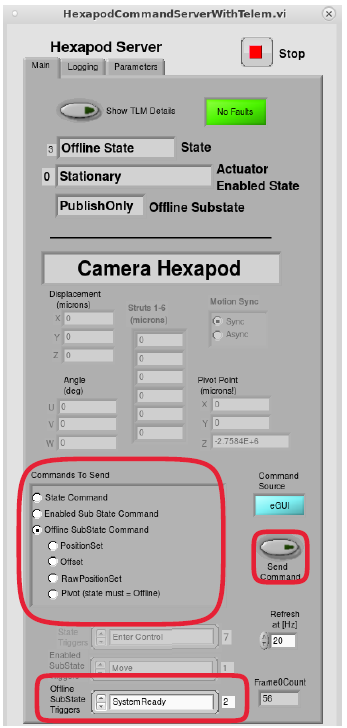
\includegraphics[width=1.79167in]{jira_imgs/1024.png}

\medskip }
\end{minipage}
\\ \cdashline{2-2}


 & Expected Result \\
 & \begin{minipage}[t]{15cm}{\footnotesize
\smallskip
The system transitions from the OfflineState/PublishOnly substate to the
OfflineState/AvailableState substate and the Command Source says
eGUI.\\[2\baselineskip]

\medskip }
\end{minipage} \\ \cdashline{2-2}

 & Actual Result \\
 & \begin{minipage}[t]{15cm}{\footnotesize
\smallskip

\medskip }
\end{minipage} \\ \cdashline{2-2}

 & Status: \textbf{ Not Executed } \\ \hline

4 & Description \\
 & \begin{minipage}[t]{15cm}
{\footnotesize
\smallskip
\textbf{OFFLINESTATE -\textgreater{} STANDBYSTATE}\\
Click on the State Command field in the Commands to Send section.\\
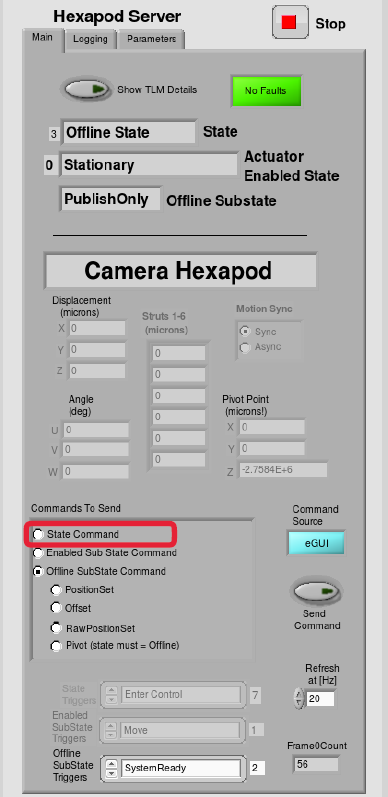
\includegraphics[width=1.79167in]{jira_imgs/1028.png}

\medskip }
\end{minipage}
\\ \cdashline{2-2}


 & Expected Result \\
 & \begin{minipage}[t]{15cm}{\footnotesize
\smallskip
The State Triggers dialogue box shown below becomes visible.\\
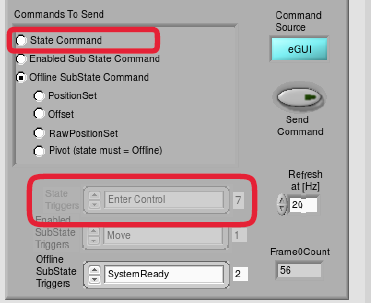
\includegraphics[width=1.79167in]{jira_imgs/1029.png}

\medskip }
\end{minipage} \\ \cdashline{2-2}

 & Actual Result \\
 & \begin{minipage}[t]{15cm}{\footnotesize
\smallskip

\medskip }
\end{minipage} \\ \cdashline{2-2}

 & Status: \textbf{ Not Executed } \\ \hline

5 & Description \\
 & \begin{minipage}[t]{15cm}
{\footnotesize
\smallskip
Scroll through the available trigger options to select ``Enter Control''
and click the Send Command button.

\medskip }
\end{minipage}
\\ \cdashline{2-2}


 & Expected Result \\
 & \begin{minipage}[t]{15cm}{\footnotesize
\smallskip
The system transitions to the Standby state and the primary state
display box at the top of the Main says Standby State.

\medskip }
\end{minipage} \\ \cdashline{2-2}

 & Actual Result \\
 & \begin{minipage}[t]{15cm}{\footnotesize
\smallskip

\medskip }
\end{minipage} \\ \cdashline{2-2}

 & Status: \textbf{ Not Executed } \\ \hline

6 & Description \\
 & \begin{minipage}[t]{15cm}
{\footnotesize
\smallskip
\textbf{STANDBYSTATE -\textgreater{} DISABLEDSTATE}\\
From the StandbyState, send a Start State command.

\medskip }
\end{minipage}
\\ \cdashline{2-2}


 & Expected Result \\
 & \begin{minipage}[t]{15cm}{\footnotesize
\smallskip
The system transitions into DisabledState and the current configuration
parameters are maintained from the default parameters or from the
previous DDS start command.~

\medskip }
\end{minipage} \\ \cdashline{2-2}

 & Actual Result \\
 & \begin{minipage}[t]{15cm}{\footnotesize
\smallskip

\medskip }
\end{minipage} \\ \cdashline{2-2}

 & Status: \textbf{ Not Executed } \\ \hline

7 & Description \\
 & \begin{minipage}[t]{15cm}
{\footnotesize
\smallskip
\textbf{DISABLEDSTATE -\textgreater{} ENABLEDSTATE}\\
From the DisabledState, send an Enable State Command.~

\medskip }
\end{minipage}
\\ \cdashline{2-2}


 & Expected Result \\
 & \begin{minipage}[t]{15cm}{\footnotesize
\smallskip
The system transitions into the EnabledState/Stationary substate, the
motor drives are enabled and and motion can be commanded.~

\medskip }
\end{minipage} \\ \cdashline{2-2}

 & Actual Result \\
 & \begin{minipage}[t]{15cm}{\footnotesize
\smallskip

\medskip }
\end{minipage} \\ \cdashline{2-2}

 & Status: \textbf{ Not Executed } \\ \hline

8 & Description \\
 & \begin{minipage}[t]{15cm}
{\footnotesize
\smallskip
\textless{}conditional state\textgreater{}\\
\textbf{FAULTSTATE}\\
If a Fault occurs in any of the other states, the system will
automatically transition to the Fault State. While in the Fault state,
send a clearError.\\
Note: If the fault that occurs goes through the interlock system, reset
the safety relay switch and send a clearError command.

\medskip }
\end{minipage}
\\ \cdashline{2-2}


 & Expected Result \\
 & \begin{minipage}[t]{15cm}{\footnotesize
\smallskip
The system transitions back to the OfflineState/PublishOnly substate.
(Go back to Step 3)

\medskip }
\end{minipage} \\ \cdashline{2-2}

 & Actual Result \\
 & \begin{minipage}[t]{15cm}{\footnotesize
\smallskip

\medskip }
\end{minipage} \\ \cdashline{2-2}

 & Status: \textbf{ Not Executed } \\ \hline

9 & Description \\
 & \begin{minipage}[t]{15cm}
{\footnotesize
\smallskip
\textbf{Section 3.1.1 of the attached Software Acceptance Test
Procedure\\
Test Sequence \#1 - Synchronous PositionSet and Move
Commands}\\[2\baselineskip]With the synchronous button enabled and in
enabled/stationary state, send a positionSet command of (0um, 0um,
200um, 0 deg, 0 deg, 0 deg) using the EUI.

\medskip }
\end{minipage}
\\ \cdashline{2-2}


 & Expected Result \\
 & \begin{minipage}[t]{15cm}{\footnotesize
\smallskip
The hexapod doesn't move.

\medskip }
\end{minipage} \\ \cdashline{2-2}

 & Actual Result \\
 & \begin{minipage}[t]{15cm}{\footnotesize
\smallskip

\medskip }
\end{minipage} \\ \cdashline{2-2}

 & Status: \textbf{ Not Executed } \\ \hline

10 & Description \\
 & \begin{minipage}[t]{15cm}
{\footnotesize
\smallskip
With the synchronous button enabled and in enabled/stationary state,
send a positionSet command of (2000um, -3500um, 200um, .01 deg, -.05deg,
.002deg) using the EUI.

\medskip }
\end{minipage}
\\ \cdashline{2-2}


 & Expected Result \\
 & \begin{minipage}[t]{15cm}{\footnotesize
\smallskip
The hexapod doesn't move.

\medskip }
\end{minipage} \\ \cdashline{2-2}

 & Actual Result \\
 & \begin{minipage}[t]{15cm}{\footnotesize
\smallskip

\medskip }
\end{minipage} \\ \cdashline{2-2}

 & Status: \textbf{ Not Executed } \\ \hline

11 & Description \\
 & \begin{minipage}[t]{15cm}
{\footnotesize
\smallskip
Send a move command using the EUI.

\medskip }
\end{minipage}
\\ \cdashline{2-2}


 & Expected Result \\
 & \begin{minipage}[t]{15cm}{\footnotesize
\smallskip
The hexapod moves to the last commanded position of (2000um, -3500um,
200um, .01 deg, -.05deg, .002deg) and the actuators complete the move at
nearly the same time as seen on the motion complete lights on the
telemetry screen.

\medskip }
\end{minipage} \\ \cdashline{2-2}

 & Actual Result \\
 & \begin{minipage}[t]{15cm}{\footnotesize
\smallskip

\medskip }
\end{minipage} \\ \cdashline{2-2}

 & Status: \textbf{ Not Executed } \\ \hline

12 & Description \\
 & \begin{minipage}[t]{15cm}
{\footnotesize
\smallskip
\textbf{Section 3.1.1 of the attached Software Acceptance Test
Procedure\\
Test Sequence \#2 - Pivot, PositionSet and Move
Commands}\\[2\baselineskip]In enabled/stationary state and at the last
commanded position of (2000um, -3500um, 200um, .01 deg, -.05deg,
.002deg), change the pivot point from the default location to (0,0,0)
using the EUI.

\medskip }
\end{minipage}
\\ \cdashline{2-2}


 & Expected Result \\
 & \begin{minipage}[t]{15cm}{\footnotesize
\smallskip
The actuator positions do not change, but the hexapod position is
(-407um, -3982um, 199um, 0.01deg, -0.05deg, 0.002deg)

\medskip }
\end{minipage} \\ \cdashline{2-2}

 & Actual Result \\
 & \begin{minipage}[t]{15cm}{\footnotesize
\smallskip

\medskip }
\end{minipage} \\ \cdashline{2-2}

 & Status: \textbf{ Not Executed } \\ \hline

13 & Description \\
 & \begin{minipage}[t]{15cm}
{\footnotesize
\smallskip
In the enabled/stationary state, send a positionSet command of (2000um,
-3500um, 200um, .01 deg, -.05deg, .002deg) using the EUI.

\medskip }
\end{minipage}
\\ \cdashline{2-2}


 & Expected Result \\
 & \begin{minipage}[t]{15cm}{\footnotesize
\smallskip
The hexapod doesn't move.

\medskip }
\end{minipage} \\ \cdashline{2-2}

 & Actual Result \\
 & \begin{minipage}[t]{15cm}{\footnotesize
\smallskip

\medskip }
\end{minipage} \\ \cdashline{2-2}

 & Status: \textbf{ Not Executed } \\ \hline

14 & Description \\
 & \begin{minipage}[t]{15cm}
{\footnotesize
\smallskip
Send a move command using the EUI.

\medskip }
\end{minipage}
\\ \cdashline{2-2}


 & Expected Result \\
 & \begin{minipage}[t]{15cm}{\footnotesize
\smallskip
The hexapod moves to the commanded position of (2000um, -3500um, 200um,
.01 deg, -.05deg, .002deg) and the actuators change position to account
for the new pivot point.

\medskip }
\end{minipage} \\ \cdashline{2-2}

 & Actual Result \\
 & \begin{minipage}[t]{15cm}{\footnotesize
\smallskip

\medskip }
\end{minipage} \\ \cdashline{2-2}

 & Status: \textbf{ Not Executed } \\ \hline

15 & Description \\
 & \begin{minipage}[t]{15cm}
{\footnotesize
\smallskip
\textbf{Section 3.1.1 of the attached Software Acceptance Test
Procedure\\
Test Sequence \#4 - Synchronous Offset and Move
Commands}\\[2\baselineskip]With the synchronous button enabled and in
enabled/stationary state, send a positionSet command of (500um, 800um,
200um, 0 deg, 0 deg, 0 deg).

\medskip }
\end{minipage}
\\ \cdashline{2-2}


 & Expected Result \\
 & \begin{minipage}[t]{15cm}{\footnotesize
\smallskip
The hexapod doesn't move.

\medskip }
\end{minipage} \\ \cdashline{2-2}

 & Actual Result \\
 & \begin{minipage}[t]{15cm}{\footnotesize
\smallskip

\medskip }
\end{minipage} \\ \cdashline{2-2}

 & Status: \textbf{ Not Executed } \\ \hline

16 & Description \\
 & \begin{minipage}[t]{15cm}
{\footnotesize
\smallskip
With the synchronous button enabled and in enabled/stationary state,
send an offset command of (0um, 0um, 2000um, 0 deg, 0 deg, 0 deg).~

\medskip }
\end{minipage}
\\ \cdashline{2-2}


 & Expected Result \\
 & \begin{minipage}[t]{15cm}{\footnotesize
\smallskip
The hexapod doesn't move.

\medskip }
\end{minipage} \\ \cdashline{2-2}

 & Actual Result \\
 & \begin{minipage}[t]{15cm}{\footnotesize
\smallskip

\medskip }
\end{minipage} \\ \cdashline{2-2}

 & Status: \textbf{ Not Executed } \\ \hline

17 & Description \\
 & \begin{minipage}[t]{15cm}
{\footnotesize
\smallskip
Send a move command.

\medskip }
\end{minipage}
\\ \cdashline{2-2}


 & Expected Result \\
 & \begin{minipage}[t]{15cm}{\footnotesize
\smallskip
The hexapod moves only 2000um in Z from the previous position and the
actuators complete the move at nearly the same time as seen on the
motion complete lights on the telemetry screen.

\medskip }
\end{minipage} \\ \cdashline{2-2}

 & Actual Result \\
 & \begin{minipage}[t]{15cm}{\footnotesize
\smallskip

\medskip }
\end{minipage} \\ \cdashline{2-2}

 & Status: \textbf{ Not Executed } \\ \hline

18 & Description \\
 & \begin{minipage}[t]{15cm}
{\footnotesize
\smallskip
\textbf{Instead of Asynchronous Test}\\
{With the synchronous button enabled and in enabled/stationary
state,}{\textbf{~}}{s}end a position set command of (0um, 0um, 0um,
0.1deg, 0deg, 0deg)

\medskip }
\end{minipage}
\\ \cdashline{2-2}


 & Expected Result \\
 & \begin{minipage}[t]{15cm}{\footnotesize
\smallskip
The hexapod doesn't move.

\medskip }
\end{minipage} \\ \cdashline{2-2}

 & Actual Result \\
 & \begin{minipage}[t]{15cm}{\footnotesize
\smallskip

\medskip }
\end{minipage} \\ \cdashline{2-2}

 & Status: \textbf{ Not Executed } \\ \hline

19 & Description \\
 & \begin{minipage}[t]{15cm}
{\footnotesize
\smallskip
Send a move command.

\medskip }
\end{minipage}
\\ \cdashline{2-2}


 & Expected Result \\
 & \begin{minipage}[t]{15cm}{\footnotesize
\smallskip
The hexapod moves to the commanded position of (0um, 0um, 0um, 0.1deg,
0deg, 0deg)

\medskip }
\end{minipage} \\ \cdashline{2-2}

 & Actual Result \\
 & \begin{minipage}[t]{15cm}{\footnotesize
\smallskip

\medskip }
\end{minipage} \\ \cdashline{2-2}

 & Status: \textbf{ Not Executed } \\ \hline

20 & Description \\
 & \begin{minipage}[t]{15cm}
{\footnotesize
\smallskip
With the synchronous button enabled and in enabled/stationary
state,\textbf{~}send a position set command of (0um, 0um, 0um, 0deg,
0.1deg, 0deg)

\medskip }
\end{minipage}
\\ \cdashline{2-2}


 & Expected Result \\
 & \begin{minipage}[t]{15cm}{\footnotesize
\smallskip
The hexapod doesn't move.

\medskip }
\end{minipage} \\ \cdashline{2-2}

 & Actual Result \\
 & \begin{minipage}[t]{15cm}{\footnotesize
\smallskip

\medskip }
\end{minipage} \\ \cdashline{2-2}

 & Status: \textbf{ Not Executed } \\ \hline

21 & Description \\
 & \begin{minipage}[t]{15cm}
{\footnotesize
\smallskip
Send a move command.

\medskip }
\end{minipage}
\\ \cdashline{2-2}


 & Expected Result \\
 & \begin{minipage}[t]{15cm}{\footnotesize
\smallskip
The hexapod moves to the commanded position of (0um, 0um, 0um, 0deg,
0.1deg, 0deg)

\medskip }
\end{minipage} \\ \cdashline{2-2}

 & Actual Result \\
 & \begin{minipage}[t]{15cm}{\footnotesize
\smallskip

\medskip }
\end{minipage} \\ \cdashline{2-2}

 & Status: \textbf{ Not Executed } \\ \hline

22 & Description \\
 & \begin{minipage}[t]{15cm}
{\footnotesize
\smallskip
With the synchronous button enabled and in enabled/stationary
state,\textbf{~}send a position set command of (0um, 0um, 0um, 0.1deg,
0.1deg, 0deg)

\medskip }
\end{minipage}
\\ \cdashline{2-2}


 & Expected Result \\
 & \begin{minipage}[t]{15cm}{\footnotesize
\smallskip
The hexapod doesn't move.

\medskip }
\end{minipage} \\ \cdashline{2-2}

 & Actual Result \\
 & \begin{minipage}[t]{15cm}{\footnotesize
\smallskip

\medskip }
\end{minipage} \\ \cdashline{2-2}

 & Status: \textbf{ Not Executed } \\ \hline

23 & Description \\
 & \begin{minipage}[t]{15cm}
{\footnotesize
\smallskip
Send a move command.

\medskip }
\end{minipage}
\\ \cdashline{2-2}


 & Expected Result \\
 & \begin{minipage}[t]{15cm}{\footnotesize
\smallskip
The hexapod moves to the commanded position of (0um, 0um, 0um, 0.1deg,
0.1deg, 0deg)

\medskip }
\end{minipage} \\ \cdashline{2-2}

 & Actual Result \\
 & \begin{minipage}[t]{15cm}{\footnotesize
\smallskip

\medskip }
\end{minipage} \\ \cdashline{2-2}

 & Status: \textbf{ Not Executed } \\ \hline

24 & Description \\
 & \begin{minipage}[t]{15cm}
{\footnotesize
\smallskip
\textbf{Section 3.1.1 of the attached Software Acceptance Test
Procedure\\
Test Sequence \#5 - Stop Commands}\\[2\baselineskip]In
enabled/stationary state, send a position set command of (0um, 0um,
5000um, 0 deg, 0 deg, 0 deg).

\medskip }
\end{minipage}
\\ \cdashline{2-2}


 & Expected Result \\
 & \begin{minipage}[t]{15cm}{\footnotesize
\smallskip
The hexapod doesn't move.

\medskip }
\end{minipage} \\ \cdashline{2-2}

 & Actual Result \\
 & \begin{minipage}[t]{15cm}{\footnotesize
\smallskip

\medskip }
\end{minipage} \\ \cdashline{2-2}

 & Status: \textbf{ Not Executed } \\ \hline

25 & Description \\
 & \begin{minipage}[t]{15cm}
{\footnotesize
\smallskip
Send a move command.

\medskip }
\end{minipage}
\\ \cdashline{2-2}


 & Expected Result \\
 & \begin{minipage}[t]{15cm}{\footnotesize
\smallskip
The hexapod starts to move to the commanded position.

\medskip }
\end{minipage} \\ \cdashline{2-2}

 & Actual Result \\
 & \begin{minipage}[t]{15cm}{\footnotesize
\smallskip

\medskip }
\end{minipage} \\ \cdashline{2-2}

 & Status: \textbf{ Not Executed } \\ \hline

26 & Description \\
 & \begin{minipage}[t]{15cm}
{\footnotesize
\smallskip
While the hexapod is moving, send a stop command.~

\medskip }
\end{minipage}
\\ \cdashline{2-2}


 & Expected Result \\
 & \begin{minipage}[t]{15cm}{\footnotesize
\smallskip
The hexapod quickly comes to a stop prior to reaching the commanded
position.

\medskip }
\end{minipage} \\ \cdashline{2-2}

 & Actual Result \\
 & \begin{minipage}[t]{15cm}{\footnotesize
\smallskip

\medskip }
\end{minipage} \\ \cdashline{2-2}

 & Status: \textbf{ Not Executed } \\ \hline

27 & Description \\
 & \begin{minipage}[t]{15cm}
{\footnotesize
\smallskip
\textbf{Section 3.3.1 EUI Tests of the attached Software Acceptance Test
Procedure}\\
At startup, confirm that the system starts in the Offline/PublishOnly
state.

\medskip }
\end{minipage}
\\ \cdashline{2-2}


 & Expected Result \\
 & \begin{minipage}[t]{15cm}{\footnotesize
\smallskip
The rotator starts in the Offline/PublishOnly state.

\medskip }
\end{minipage} \\ \cdashline{2-2}

 & Actual Result \\
 & \begin{minipage}[t]{15cm}{\footnotesize
\smallskip

\medskip }
\end{minipage} \\ \cdashline{2-2}

 & Status: \textbf{ Not Executed } \\ \hline

28 & Description \\
 & \begin{minipage}[t]{15cm}
{\footnotesize
\smallskip
Send an offline substate trigger of systemReady.

\medskip }
\end{minipage}
\\ \cdashline{2-2}


 & Expected Result \\
 & \begin{minipage}[t]{15cm}{\footnotesize
\smallskip
The system transitions into the Offline/Available substate.

\medskip }
\end{minipage} \\ \cdashline{2-2}

 & Actual Result \\
 & \begin{minipage}[t]{15cm}{\footnotesize
\smallskip

\medskip }
\end{minipage} \\ \cdashline{2-2}

 & Status: \textbf{ Not Executed } \\ \hline

29 & Description \\
 & \begin{minipage}[t]{15cm}
{\footnotesize
\smallskip
Send an EnterControl trigger.

\medskip }
\end{minipage}
\\ \cdashline{2-2}


 & Expected Result \\
 & \begin{minipage}[t]{15cm}{\footnotesize
\smallskip
The system transitions from Offline/Available to Standby state.

\medskip }
\end{minipage} \\ \cdashline{2-2}

 & Actual Result \\
 & \begin{minipage}[t]{15cm}{\footnotesize
\smallskip

\medskip }
\end{minipage} \\ \cdashline{2-2}

 & Status: \textbf{ Not Executed } \\ \hline

30 & Description \\
 & \begin{minipage}[t]{15cm}
{\footnotesize
\smallskip
Send a Start trigger.

\medskip }
\end{minipage}
\\ \cdashline{2-2}


 & Expected Result \\
 & \begin{minipage}[t]{15cm}{\footnotesize
\smallskip
The system transitions from Standby to Disabled state.

\medskip }
\end{minipage} \\ \cdashline{2-2}

 & Actual Result \\
 & \begin{minipage}[t]{15cm}{\footnotesize
\smallskip

\medskip }
\end{minipage} \\ \cdashline{2-2}

 & Status: \textbf{ Not Executed } \\ \hline

31 & Description \\
 & \begin{minipage}[t]{15cm}
{\footnotesize
\smallskip
Send an Enable trigger.

\medskip }
\end{minipage}
\\ \cdashline{2-2}


 & Expected Result \\
 & \begin{minipage}[t]{15cm}{\footnotesize
\smallskip
The system transitions from Disabled to Enabled state.

\medskip }
\end{minipage} \\ \cdashline{2-2}

 & Actual Result \\
 & \begin{minipage}[t]{15cm}{\footnotesize
\smallskip

\medskip }
\end{minipage} \\ \cdashline{2-2}

 & Status: \textbf{ Not Executed } \\ \hline

32 & Description \\
 & \begin{minipage}[t]{15cm}
{\footnotesize
\smallskip
Send a Disable trigger.

\medskip }
\end{minipage}
\\ \cdashline{2-2}


 & Expected Result \\
 & \begin{minipage}[t]{15cm}{\footnotesize
\smallskip
The system transitions from Enabled to Disabled state.

\medskip }
\end{minipage} \\ \cdashline{2-2}

 & Actual Result \\
 & \begin{minipage}[t]{15cm}{\footnotesize
\smallskip

\medskip }
\end{minipage} \\ \cdashline{2-2}

 & Status: \textbf{ Not Executed } \\ \hline

33 & Description \\
 & \begin{minipage}[t]{15cm}
{\footnotesize
\smallskip
Send a Standby trigger.

\medskip }
\end{minipage}
\\ \cdashline{2-2}


 & Expected Result \\
 & \begin{minipage}[t]{15cm}{\footnotesize
\smallskip
The system transitions from Disabled state to Standby state.

\medskip }
\end{minipage} \\ \cdashline{2-2}

 & Actual Result \\
 & \begin{minipage}[t]{15cm}{\footnotesize
\smallskip

\medskip }
\end{minipage} \\ \cdashline{2-2}

 & Status: \textbf{ Not Executed } \\ \hline

34 & Description \\
 & \begin{minipage}[t]{15cm}
{\footnotesize
\smallskip
Send a exitControl trigger.

\medskip }
\end{minipage}
\\ \cdashline{2-2}


 & Expected Result \\
 & \begin{minipage}[t]{15cm}{\footnotesize
\smallskip
The system transitions from Standby state to Offline state.

\medskip }
\end{minipage} \\ \cdashline{2-2}

 & Actual Result \\
 & \begin{minipage}[t]{15cm}{\footnotesize
\smallskip

\medskip }
\end{minipage} \\ \cdashline{2-2}

 & Status: \textbf{ Not Executed } \\ \hline

35 & Description \\
 & \begin{minipage}[t]{15cm}
{\footnotesize
\smallskip
Return to the Enabled state and trip the safety interlock switch.

\medskip }
\end{minipage}
\\ \cdashline{2-2}


 & Expected Result \\
 & \begin{minipage}[t]{15cm}{\footnotesize
\smallskip
The system transitions to Fault state.

\medskip }
\end{minipage} \\ \cdashline{2-2}

 & Actual Result \\
 & \begin{minipage}[t]{15cm}{\footnotesize
\smallskip

\medskip }
\end{minipage} \\ \cdashline{2-2}

 & Status: \textbf{ Not Executed } \\ \hline

36 & Description \\
 & \begin{minipage}[t]{15cm}
{\footnotesize
\smallskip
Reset the safety interlock and send a ClearError trigger.

\medskip }
\end{minipage}
\\ \cdashline{2-2}


 & Expected Result \\
 & \begin{minipage}[t]{15cm}{\footnotesize
\smallskip
The system transitions from Fault state to Offline state

\medskip }
\end{minipage} \\ \cdashline{2-2}

 & Actual Result \\
 & \begin{minipage}[t]{15cm}{\footnotesize
\smallskip

\medskip }
\end{minipage} \\ \cdashline{2-2}

 & Status: \textbf{ Not Executed } \\ \hline

37 & Description \\
 & \begin{minipage}[t]{15cm}
{\footnotesize
\smallskip
\textbf{Section 4.1 Hexapod Events of the attached Software Acceptance
Test Procedure}\\[2\baselineskip]In the Enabled/Stationary state, unplug
a motor encoder cable for one of the actuators.

\medskip }
\end{minipage}
\\ \cdashline{2-2}

 & Test Data \\
 & \begin{minipage}[t]{15cm}{\footnotesize
\smallskip
\textbf{Deviation:~}Perform the following set of steps using the EUI
instead of the DDS and verify the events are displayed on the EUI.

\medskip }
\end{minipage} \\ \cdashline{2-2}

 & Expected Result \\
 & \begin{minipage}[t]{15cm}{\footnotesize
\smallskip
A Drive Fault error event is created and the system transitions to Fault
state.

\medskip }
\end{minipage} \\ \cdashline{2-2}

 & Actual Result \\
 & \begin{minipage}[t]{15cm}{\footnotesize
\smallskip

\medskip }
\end{minipage} \\ \cdashline{2-2}

 & Status: \textbf{ Not Executed } \\ \hline

38 & Description \\
 & \begin{minipage}[t]{15cm}
{\footnotesize
\smallskip
In the Enabled/Stationary state, unplug a linear encoder cable for one
of the actuators.~

\medskip }
\end{minipage}
\\ \cdashline{2-2}


 & Expected Result \\
 & \begin{minipage}[t]{15cm}{\footnotesize
\smallskip
A Drive Fault error event is created and the system transitions to Fault
state.

\medskip }
\end{minipage} \\ \cdashline{2-2}

 & Actual Result \\
 & \begin{minipage}[t]{15cm}{\footnotesize
\smallskip

\medskip }
\end{minipage} \\ \cdashline{2-2}

 & Status: \textbf{ Not Executed } \\ \hline

39 & Description \\
 & \begin{minipage}[t]{15cm}
{\footnotesize
\smallskip
Unplug a motor power cable from one of the actuators and command a
PositionSet/Move.~

\medskip }
\end{minipage}
\\ \cdashline{2-2}


 & Expected Result \\
 & \begin{minipage}[t]{15cm}{\footnotesize
\smallskip
A Following Error event is created and the system transitions to Fault
state.

\medskip }
\end{minipage} \\ \cdashline{2-2}

 & Actual Result \\
 & \begin{minipage}[t]{15cm}{\footnotesize
\smallskip

\medskip }
\end{minipage} \\ \cdashline{2-2}

 & Status: \textbf{ Not Executed } \\ \hline

40 & Description \\
 & \begin{minipage}[t]{15cm}
{\footnotesize
\smallskip
Activate an extension limit switch on one of the actuators by removing
the limit switch cover and manually tripping.~

\medskip }
\end{minipage}
\\ \cdashline{2-2}


 & Expected Result \\
 & \begin{minipage}[t]{15cm}{\footnotesize
\smallskip
An Extended Limit Switch error event is created and the system
transitions into Fault state.

\medskip }
\end{minipage} \\ \cdashline{2-2}

 & Actual Result \\
 & \begin{minipage}[t]{15cm}{\footnotesize
\smallskip

\medskip }
\end{minipage} \\ \cdashline{2-2}

 & Status: \textbf{ Not Executed } \\ \hline

41 & Description \\
 & \begin{minipage}[t]{15cm}
{\footnotesize
\smallskip
Activate a retraction limit switch on one of the actuators by removing
the limit switch cover and manually tripping.

\medskip }
\end{minipage}
\\ \cdashline{2-2}


 & Expected Result \\
 & \begin{minipage}[t]{15cm}{\footnotesize
\smallskip
A Retracted Limit Switch error event is created and the system
transitions into Fault state.

\medskip }
\end{minipage} \\ \cdashline{2-2}

 & Actual Result \\
 & \begin{minipage}[t]{15cm}{\footnotesize
\smallskip

\medskip }
\end{minipage} \\ \cdashline{2-2}

 & Status: \textbf{ Not Executed } \\ \hline

42 & Description \\
 & \begin{minipage}[t]{15cm}
{\footnotesize
\smallskip
Unplug the Ethercat cable between the control PC and the first Copley
XE2 drive.

\medskip }
\end{minipage}
\\ \cdashline{2-2}


 & Expected Result \\
 & \begin{minipage}[t]{15cm}{\footnotesize
\smallskip
An Ethercat Lost event is created and the system transitions to Fault
state.

\medskip }
\end{minipage} \\ \cdashline{2-2}

 & Actual Result \\
 & \begin{minipage}[t]{15cm}{\footnotesize
\smallskip

\medskip }
\end{minipage} \\ \cdashline{2-2}

 & Status: \textbf{ Not Executed } \\ \hline

\end{longtable}

\paragraph{Test Case LVV-T1600 - Integration of Camera Hexapod with SAL 4.0 (LSST)
 }\mbox{}\\

Open  \href{https://jira.lsstcorp.org/secure/Tests.jspa#/testCase/LVV-T1600}{\textit{ LVV-T1600 } }
test case in Jira.

The objective of this test case is to re-verify the functional
requirements of the camera hexapod's software, after shipment of the
hardware from the vendor's facility to the Summit, as defined in \citeds{LTS-206}
and \citeds{LTS-160}. This test case will only exercise the functionality that
was executed previously and meets the following criteria:

\begin{itemize}
\tightlist
\item
  Only requires the camera hexapod to be operable
\item
  Only requires command through the CSC after the cRIO is switched from
  GUI mode to DDS mode
\item
  Only requires testing of the synchronous mode

  \begin{itemize}
  \tightlist
  \item
    \textbf{Asynchronous mode is not a standard mode of operation}
  \end{itemize}
\item
  Does \textbf{NOT} require the camera hexapod to be loaded with the
  camera simulated mass or actual camera hardware
\end{itemize}

The software functional requirements were previously verified during the
test campaign by the vendor at the vendor's facility and accepted by
LSST during the Factory Acceptance Test review. The test procedure used
during the vendor's acceptance testing is the \emph{LSST
Hexapods-Rotator Software Acceptance Test Procedure} which is attached
to this test case. The test steps of this test case are taken directly
from that document on how to perform the test in a similar way as was
performed previously and includes changes noted by the
vendor.\\[2\baselineskip]See the attached \emph{LSST Rotator Hexapod's
Manual} for more information on how to operate the hexapod.


\textbf{ Preconditions}:\\
Prior to the execution of this test case to re-verify the Camera Hexapod
hardware functional requirements, the following Summit tasks must be
completed:

\begin{itemize}
\tightlist
\item
  The Hexapod has been installed on the camera cart

  \begin{itemize}
  \tightlist
  \item
    \url{https://jira.lsstcorp.org/browse/SUMMIT-3224}
  \end{itemize}
\item
  The Hexapod Controller has been deployed on the summit

  \begin{itemize}
  \tightlist
  \item
    \url{https://jira.lsstcorp.org/browse/SUMMIT-3229}
  \end{itemize}
\item
  Boxes for the Hexapod have been transported to the 3rd level

  \begin{itemize}
  \tightlist
  \item
    \url{https://jira.lsstcorp.org/browse/SUMMIT-3230}
  \end{itemize}
\item
  All Hexapod cables and cabinets have been prepared for integration
  with camera cart

  \begin{itemize}
  \tightlist
  \item
    \url{https://jira.lsstcorp.org/browse/SUMMIT-3231}
  \end{itemize}
\item
  The offset has been installed onto the integrating structure

  \begin{itemize}
  \tightlist
  \item
    \url{https://jira.lsstcorp.org/browse/SUMMIT-3293}
  \end{itemize}
\item
  The Camera Hexapod electrical connections have been tested

  \begin{itemize}
  \tightlist
  \item
    \url{https://jira.lsstcorp.org/browse/SUMMIT-3294}
  \end{itemize}
\end{itemize}


Execution status: {\bf Not Executed }

Final comment:\\


Detailed steps results:

\begin{longtable}{p{1cm}p{15cm}}
\hline
{Step} & Step Details\\ \hline
1 & Description \\
 & \begin{minipage}[t]{15cm}
{\footnotesize
\smallskip
\textbf{STARTING THE EUI}\\[2\baselineskip]Double click the Rotator GUI
Viewer desktop icon on the computer.

\begin{itemize}
\tightlist
\item
  This can be done on the Dell Management PC or another computer on the
  same network
\end{itemize}

\medskip }
\end{minipage}
\\ \cdashline{2-2}


 & Expected Result \\
 & \begin{minipage}[t]{15cm}{\footnotesize
\smallskip
A prompt to enter a password is shown.~

\medskip }
\end{minipage} \\ \cdashline{2-2}

 & Actual Result \\
 & \begin{minipage}[t]{15cm}{\footnotesize
\smallskip

\medskip }
\end{minipage} \\ \cdashline{2-2}

 & Status: \textbf{ Not Executed } \\ \hline

2 & Description \\
 & \begin{minipage}[t]{15cm}
{\footnotesize
\smallskip
Enter the password ``lsst-vnc''

\begin{itemize}
\tightlist
\item
  If the EUI isn't automatically up and running when the VNC opens,
  double click on the Rotator-eGUI icon on the VNC viewer
\end{itemize}

\medskip }
\end{minipage}
\\ \cdashline{2-2}


 & Expected Result \\
 & \begin{minipage}[t]{15cm}{\footnotesize
\smallskip
The EUI is in the Offline State/PublishOnly substate and is able to
publish through SAL but cannot receive commands.

\medskip }
\end{minipage} \\ \cdashline{2-2}

 & Actual Result \\
 & \begin{minipage}[t]{15cm}{\footnotesize
\smallskip

\medskip }
\end{minipage} \\ \cdashline{2-2}

 & Status: \textbf{ Not Executed } \\ \hline

3 & Description \\
 & \begin{minipage}[t]{15cm}
{\footnotesize
\smallskip
\textbf{OFFLINESTATE/PUBLISHONLY -\textgreater{}
OFFLINESTATE/AVAILABLESTATE}\\
On the Main tab, select the ``Offline SubState Cmd'' field in the
Commands to Send section, set the Offline SubState Triggers to ``System
Ready'' and click on the Send Command button.\\
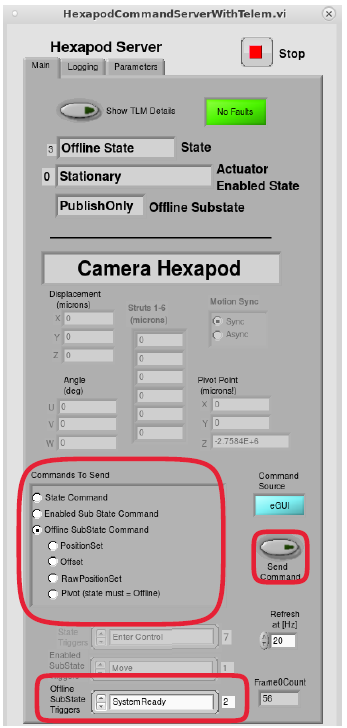
\includegraphics[width=1.79167in]{jira_imgs/1024.png}

\medskip }
\end{minipage}
\\ \cdashline{2-2}


 & Expected Result \\
 & \begin{minipage}[t]{15cm}{\footnotesize
\smallskip
The system transitions from the OfflineState/PublishOnly substate to the
OfflineState/AvailableState substate.\\[2\baselineskip]

\medskip }
\end{minipage} \\ \cdashline{2-2}

 & Actual Result \\
 & \begin{minipage}[t]{15cm}{\footnotesize
\smallskip

\medskip }
\end{minipage} \\ \cdashline{2-2}

 & Status: \textbf{ Not Executed } \\ \hline

4 & Description \\
 & \begin{minipage}[t]{15cm}
{\footnotesize
\smallskip
\textbf{SWITCHING TO DDS MODE}\\
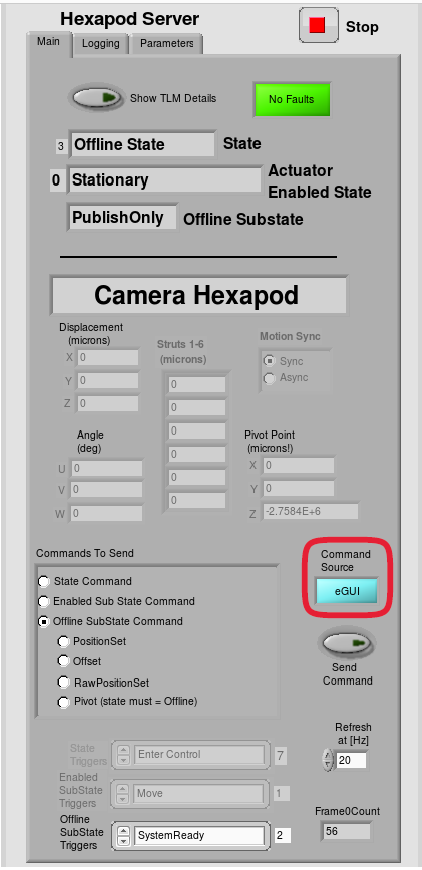
\includegraphics[width=1.68750in]{jira_imgs/1025.png}If the Command
Source does not show DDS, go to the Parameters tab, select DDS under the
Command Source and click the Set Cmd Source button.\\
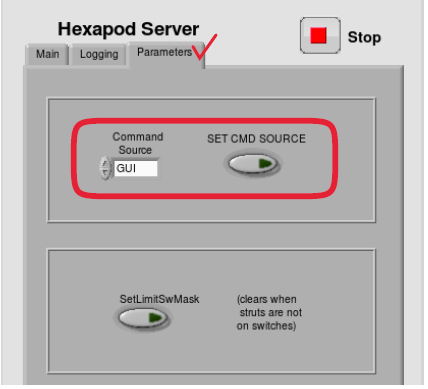
\includegraphics[width=2.34375in]{jira_imgs/1026.png}\textbf{Note:~If
the GUI is used after being set to DDS mode, the system will switch back
the Command Source to GUI and ignore any DDS commands. The Command
Source must show DDS in order to receive DDS commands.}

\medskip }
\end{minipage}
\\ \cdashline{2-2}


 & Expected Result \\
 & \begin{minipage}[t]{15cm}{\footnotesize
\smallskip
The system is capable of receiving/responding to DDS commands.

\medskip }
\end{minipage} \\ \cdashline{2-2}

 & Actual Result \\
 & \begin{minipage}[t]{15cm}{\footnotesize
\smallskip

\medskip }
\end{minipage} \\ \cdashline{2-2}

 & Status: \textbf{ Not Executed } \\ \hline

5 & Description \\
 & \begin{minipage}[t]{15cm}
{\footnotesize
\smallskip
\textbf{OFFLINESTATE -\textgreater{} STANDBYSTATE}\\
The system receives an enterControl State Transition command through
DDS.

\medskip }
\end{minipage}
\\ \cdashline{2-2}


 & Expected Result \\
 & \begin{minipage}[t]{15cm}{\footnotesize
\smallskip
The system transitions into the StandbyState and is capable of
receiving/responding to DDS commands.

\medskip }
\end{minipage} \\ \cdashline{2-2}

 & Actual Result \\
 & \begin{minipage}[t]{15cm}{\footnotesize
\smallskip

\medskip }
\end{minipage} \\ \cdashline{2-2}

 & Status: \textbf{ Not Executed } \\ \hline

6 & Description \\
 & \begin{minipage}[t]{15cm}
{\footnotesize
\smallskip
\textbf{STANDBYSTATE -\textgreater{} DISABLEDSTATE}\\
From the StandbyState, send a start command through the DDS.

\medskip }
\end{minipage}
\\ \cdashline{2-2}


 & Expected Result \\
 & \begin{minipage}[t]{15cm}{\footnotesize
\smallskip
The system transitions into DisabledState after receiving/responding to
DDS command and the wrapper in the PXI real time controller looks for
the configuration file.\\[2\baselineskip]If the configuration file is
invalid or out of range, the system will transition into a Fault State

\medskip }
\end{minipage} \\ \cdashline{2-2}

 & Actual Result \\
 & \begin{minipage}[t]{15cm}{\footnotesize
\smallskip

\medskip }
\end{minipage} \\ \cdashline{2-2}

 & Status: \textbf{ Not Executed } \\ \hline

7 & Description \\
 & \begin{minipage}[t]{15cm}
{\footnotesize
\smallskip
\textbf{DISABLEDSTATE -\textgreater{} ENABLEDSTATE}\\
From the DisabledState, send an enable state command through the DDS.\\
\textbf{}

\medskip }
\end{minipage}
\\ \cdashline{2-2}


 & Expected Result \\
 & \begin{minipage}[t]{15cm}{\footnotesize
\smallskip
The system transitions into the EnabledState/Stationary substate, the
motor drives are enabled, motor brakes are released and the system is
capable of receiving/responding to DDS commands.\\[2\baselineskip]

\medskip }
\end{minipage} \\ \cdashline{2-2}

 & Actual Result \\
 & \begin{minipage}[t]{15cm}{\footnotesize
\smallskip

\medskip }
\end{minipage} \\ \cdashline{2-2}

 & Status: \textbf{ Not Executed } \\ \hline

8 & Description \\
 & \begin{minipage}[t]{15cm}
{\footnotesize
\smallskip
\textbf{FAULTSTATE}\\
If a Fault occurs in any of the other states, the system will
automatically transition to the Fault State. While in the Fault state,
send a clearError command through the DDS.\\
Note: If the fault that occurs goes through the interlock system, reset
the safety relay switch and send a clearError command.

\medskip }
\end{minipage}
\\ \cdashline{2-2}


 & Expected Result \\
 & \begin{minipage}[t]{15cm}{\footnotesize
\smallskip
The system transitions back to the OfflineState/PublishOnly substate and
is not capable of receiving/responding to DDS commands. (Go back to Step
3)

\medskip }
\end{minipage} \\ \cdashline{2-2}

 & Actual Result \\
 & \begin{minipage}[t]{15cm}{\footnotesize
\smallskip

\medskip }
\end{minipage} \\ \cdashline{2-2}

 & Status: \textbf{ Not Executed } \\ \hline

9 & Description \\
 & \begin{minipage}[t]{15cm}
{\footnotesize
\smallskip
\textbf{{MOVE TEST}}\\
\textbf{Section 3.1.2 of the attached Software Acceptance Test
Procedure\\
Test Sequence \#1 - Synchronous PositionSet and Move Commands}\\
In enabled/stationary state, send a positionSet command of (0um, 0um,
200um, 0 deg, 0 deg, 0 deg, s).

\medskip }
\end{minipage}
\\ \cdashline{2-2}


 & Expected Result \\
 & \begin{minipage}[t]{15cm}{\footnotesize
\smallskip
The hexapod does not move.

\medskip }
\end{minipage} \\ \cdashline{2-2}

 & Actual Result \\
 & \begin{minipage}[t]{15cm}{\footnotesize
\smallskip

\medskip }
\end{minipage} \\ \cdashline{2-2}

 & Status: \textbf{ Not Executed } \\ \hline

10 & Description \\
 & \begin{minipage}[t]{15cm}
{\footnotesize
\smallskip
In enabled/stationary state, send a positionSet command of (2000um,
-3500um, 200um, 0.01deg, -.05deg, 0.002deg).

\medskip }
\end{minipage}
\\ \cdashline{2-2}


 & Expected Result \\
 & \begin{minipage}[t]{15cm}{\footnotesize
\smallskip
The hexapod does not move

\medskip }
\end{minipage} \\ \cdashline{2-2}

 & Actual Result \\
 & \begin{minipage}[t]{15cm}{\footnotesize
\smallskip

\medskip }
\end{minipage} \\ \cdashline{2-2}

 & Status: \textbf{ Not Executed } \\ \hline

11 & Description \\
 & \begin{minipage}[t]{15cm}
{\footnotesize
\smallskip
Send a move command.

\medskip }
\end{minipage}
\\ \cdashline{2-2}


 & Expected Result \\
 & \begin{minipage}[t]{15cm}{\footnotesize
\smallskip
The hexapod moves to (2000um, -3500um, 200um, 0.01deg, -.05deg,
0.002deg), an inPosition event is generated when the move is complete
and the actuators complete the move at nearly the same time.

\medskip }
\end{minipage} \\ \cdashline{2-2}

 & Actual Result \\
 & \begin{minipage}[t]{15cm}{\footnotesize
\smallskip

\medskip }
\end{minipage} \\ \cdashline{2-2}

 & Status: \textbf{ Not Executed } \\ \hline

12 & Description \\
 & \begin{minipage}[t]{15cm}
{\footnotesize
\smallskip
Record the corresponding DDS events that were generated.

\medskip }
\end{minipage}
\\ \cdashline{2-2}


 & Expected Result \\
 & \begin{minipage}[t]{15cm}{\footnotesize
\smallskip
The controllerState.enabledSubstate goes to MOVING\_POINT\_TO\_POINT
when the move begins and STATIONARY when the move ends.

\medskip }
\end{minipage} \\ \cdashline{2-2}

 & Actual Result \\
 & \begin{minipage}[t]{15cm}{\footnotesize
\smallskip

\medskip }
\end{minipage} \\ \cdashline{2-2}

 & Status: \textbf{ Not Executed } \\ \hline

13 & Description \\
 & \begin{minipage}[t]{15cm}
{\footnotesize
\smallskip
\textbf{Section 3.1.2 of the attached Software Acceptance Test
Procedure\\
Test Sequence \#5 - Stop Commands}\\
In the enabled/stationary state, send a position set command of (0um,
0um, 5000um, 0deg, 0deg, 0deg)

\medskip }
\end{minipage}
\\ \cdashline{2-2}


 & Expected Result \\
 & \begin{minipage}[t]{15cm}{\footnotesize
\smallskip
The hexapod doesn't move.

\medskip }
\end{minipage} \\ \cdashline{2-2}

 & Actual Result \\
 & \begin{minipage}[t]{15cm}{\footnotesize
\smallskip

\medskip }
\end{minipage} \\ \cdashline{2-2}

 & Status: \textbf{ Not Executed } \\ \hline

14 & Description \\
 & \begin{minipage}[t]{15cm}
{\footnotesize
\smallskip
Send move command.

\medskip }
\end{minipage}
\\ \cdashline{2-2}


 & Expected Result \\
 & \begin{minipage}[t]{15cm}{\footnotesize
\smallskip
The hexapod begins to move.

\medskip }
\end{minipage} \\ \cdashline{2-2}

 & Actual Result \\
 & \begin{minipage}[t]{15cm}{\footnotesize
\smallskip

\medskip }
\end{minipage} \\ \cdashline{2-2}

 & Status: \textbf{ Not Executed } \\ \hline

15 & Description \\
 & \begin{minipage}[t]{15cm}
{\footnotesize
\smallskip
Before the hexapod completes its movement, send a stop command.

\medskip }
\end{minipage}
\\ \cdashline{2-2}


 & Expected Result \\
 & \begin{minipage}[t]{15cm}{\footnotesize
\smallskip
The hexapod stops before reaching the previously commanded position and
no inPosition event is generated.~

\medskip }
\end{minipage} \\ \cdashline{2-2}

 & Actual Result \\
 & \begin{minipage}[t]{15cm}{\footnotesize
\smallskip

\medskip }
\end{minipage} \\ \cdashline{2-2}

 & Status: \textbf{ Not Executed } \\ \hline

16 & Description \\
 & \begin{minipage}[t]{15cm}
{\footnotesize
\smallskip
Record the corresponding DDS events that were generated.

\medskip }
\end{minipage}
\\ \cdashline{2-2}


 & Expected Result \\
 & \begin{minipage}[t]{15cm}{\footnotesize
\smallskip
The controllerState.enabledSubstate goes to CONTROLLED\_STOPPING when
the stop is requested, then STATIONARY when the hexapod has halted.

\medskip }
\end{minipage} \\ \cdashline{2-2}

 & Actual Result \\
 & \begin{minipage}[t]{15cm}{\footnotesize
\smallskip

\medskip }
\end{minipage} \\ \cdashline{2-2}

 & Status: \textbf{ Not Executed } \\ \hline

17 & Description \\
 & \begin{minipage}[t]{15cm}
{\footnotesize
\smallskip
\textbf{Section 3.1.2 of the attached Software Acceptance Test
Procedure\\
Test Sequence \#9 - positionSet and moveLUT}\\
In enabled/stationary state, send a positionSet command of (0um, 0um,
200um, 0deg, 0deg, 0deg)

\medskip }
\end{minipage}
\\ \cdashline{2-2}


 & Expected Result \\
 & \begin{minipage}[t]{15cm}{\footnotesize
\smallskip
The hexapod doesn't move.

\medskip }
\end{minipage} \\ \cdashline{2-2}

 & Actual Result \\
 & \begin{minipage}[t]{15cm}{\footnotesize
\smallskip

\medskip }
\end{minipage} \\ \cdashline{2-2}

 & Status: \textbf{ Not Executed } \\ \hline

18 & Description \\
 & \begin{minipage}[t]{15cm}
{\footnotesize
\smallskip
In enabled/stationary state, send a positionSet command of (0um, 0um,
800um, 0deg, 0deg, 0deg)

\medskip }
\end{minipage}
\\ \cdashline{2-2}


 & Expected Result \\
 & \begin{minipage}[t]{15cm}{\footnotesize
\smallskip
The hexapod doesn't move.

\medskip }
\end{minipage} \\ \cdashline{2-2}

 & Actual Result \\
 & \begin{minipage}[t]{15cm}{\footnotesize
\smallskip

\medskip }
\end{minipage} \\ \cdashline{2-2}

 & Status: \textbf{ Not Executed } \\ \hline

19 & Description \\
 & \begin{minipage}[t]{15cm}
{\footnotesize
\smallskip
Send a moveLUT (180deg, 60deg, and 10deg) command

\medskip }
\end{minipage}
\\ \cdashline{2-2}


 & Expected Result \\
 & \begin{minipage}[t]{15cm}{\footnotesize
\smallskip
The hexapod moves to a different position than (0um, 0um, 800um, 0deg,
0deg, 0deg) and the actuators complete the move at nearly the same time.

\medskip }
\end{minipage} \\ \cdashline{2-2}

 & Actual Result \\
 & \begin{minipage}[t]{15cm}{\footnotesize
\smallskip

\medskip }
\end{minipage} \\ \cdashline{2-2}

 & Status: \textbf{ Not Executed } \\ \hline

20 & Description \\
 & \begin{minipage}[t]{15cm}
{\footnotesize
\smallskip
{\textbf{OFFSET TEST}}\\
\textbf{Section 3.1.2 of the attached Software Acceptance Test
Procedure\\
Test Sequence \#4 - Synchronous Offset and Move Commands}\\
In enabled/stationary state, send a position command of (500um, 800um,
200um, 0deg, 0deg, 0deg)

\medskip }
\end{minipage}
\\ \cdashline{2-2}

 & Test Data \\
 & \begin{minipage}[t]{15cm}{\footnotesize
\smallskip


\medskip }
\end{minipage} \\ \cdashline{2-2}

 & Expected Result \\
 & \begin{minipage}[t]{15cm}{\footnotesize
\smallskip
The hexapod doesn't move.

\medskip }
\end{minipage} \\ \cdashline{2-2}

 & Actual Result \\
 & \begin{minipage}[t]{15cm}{\footnotesize
\smallskip

\medskip }
\end{minipage} \\ \cdashline{2-2}

 & Status: \textbf{ Not Executed } \\ \hline

21 & Description \\
 & \begin{minipage}[t]{15cm}
{\footnotesize
\smallskip
In enabled/stationary state, send an offset command of (0um, 0um,
2000um, 0deg, 0deg, 0deg).

\medskip }
\end{minipage}
\\ \cdashline{2-2}


 & Expected Result \\
 & \begin{minipage}[t]{15cm}{\footnotesize
\smallskip
The hexapod doesn't move.

\medskip }
\end{minipage} \\ \cdashline{2-2}

 & Actual Result \\
 & \begin{minipage}[t]{15cm}{\footnotesize
\smallskip

\medskip }
\end{minipage} \\ \cdashline{2-2}

 & Status: \textbf{ Not Executed } \\ \hline

22 & Description \\
 & \begin{minipage}[t]{15cm}
{\footnotesize
\smallskip
Send a move command.~

\medskip }
\end{minipage}
\\ \cdashline{2-2}


 & Expected Result \\
 & \begin{minipage}[t]{15cm}{\footnotesize
\smallskip
The hexapod moves only 2000um in Z from the previous position, the
inPosition event is generated when the move is complete and the
actuators complete the move at nearly the same time.

\medskip }
\end{minipage} \\ \cdashline{2-2}

 & Actual Result \\
 & \begin{minipage}[t]{15cm}{\footnotesize
\smallskip

\medskip }
\end{minipage} \\ \cdashline{2-2}

 & Status: \textbf{ Not Executed } \\ \hline

23 & Description \\
 & \begin{minipage}[t]{15cm}
{\footnotesize
\smallskip
Record the corresponding DDS events that were generated.

\medskip }
\end{minipage}
\\ \cdashline{2-2}


 & Expected Result \\
 & \begin{minipage}[t]{15cm}{\footnotesize
\smallskip
\begin{itemize}
\tightlist
\item
  The controllerState.enabledSubstate goes to MOVING\_POINT\_TO\_POINT
  when the move begins and STATIONARY when the move ends
\item
  The inPosition event is True when the move finishes, then False when
  the enabledSubstate goes back to STATIONARY.
\end{itemize}

\medskip }
\end{minipage} \\ \cdashline{2-2}

 & Actual Result \\
 & \begin{minipage}[t]{15cm}{\footnotesize
\smallskip

\medskip }
\end{minipage} \\ \cdashline{2-2}

 & Status: \textbf{ Not Executed } \\ \hline

24 & Description \\
 & \begin{minipage}[t]{15cm}
{\footnotesize
\smallskip
\textbf{Section 3.1.2 of the attached Software Acceptance Test
Procedure\\
Test Sequence \#2 -Pivot, PositionSet and Move Commands}\\
In enabled/stationary state and at the last commanded position, send a
pivot command of (0, 0, 0).

\medskip }
\end{minipage}
\\ \cdashline{2-2}

 & Test Data \\
 & \begin{minipage}[t]{15cm}{\footnotesize
\smallskip
\textbf{{This test step goes along with how if we have a pivot point not
at the origin, the commanded position will be the certain dimensions
from where it currently is. Discuss with Te-wei.}}\\[2\baselineskip]

\medskip }
\end{minipage} \\ \cdashline{2-2}

 & Expected Result \\
 & \begin{minipage}[t]{15cm}{\footnotesize
\smallskip
The actuator positions do not change, but the hexapod position does
change.

\medskip }
\end{minipage} \\ \cdashline{2-2}

 & Actual Result \\
 & \begin{minipage}[t]{15cm}{\footnotesize
\smallskip

\medskip }
\end{minipage} \\ \cdashline{2-2}

 & Status: \textbf{ Not Executed } \\ \hline

25 & Description \\
 & \begin{minipage}[t]{15cm}
{\footnotesize
\smallskip
\textbf{{Ask Te-wei if there are certain offset commands to issue to
test before the move command.}}

\medskip }
\end{minipage}
\\ \cdashline{2-2}


 & Expected Result \\
 & \begin{minipage}[t]{15cm}{\footnotesize
\smallskip

\medskip }
\end{minipage} \\ \cdashline{2-2}

 & Actual Result \\
 & \begin{minipage}[t]{15cm}{\footnotesize
\smallskip

\medskip }
\end{minipage} \\ \cdashline{2-2}

 & Status: \textbf{ Not Executed } \\ \hline

26 & Description \\
 & \begin{minipage}[t]{15cm}
{\footnotesize
\smallskip
\textbf{{CONFIGURE LIMITS TEST}}\\
\textbf{Section 3.1.2 of the attached Software Acceptance Test
Procedure\\
Test Sequence \#6 - configureLimits Command}\\
In enabled/stationary state, send a configureLimits command of (12000um,
-1000um, 1000um, 0.1, -0.1, 0.05)

\medskip }
\end{minipage}
\\ \cdashline{2-2}


 & Expected Result \\
 & \begin{minipage}[t]{15cm}{\footnotesize
\smallskip
The command is rejected for being outside acceptable limits.

\medskip }
\end{minipage} \\ \cdashline{2-2}

 & Actual Result \\
 & \begin{minipage}[t]{15cm}{\footnotesize
\smallskip

\medskip }
\end{minipage} \\ \cdashline{2-2}

 & Status: \textbf{ Not Executed } \\ \hline

27 & Description \\
 & \begin{minipage}[t]{15cm}
{\footnotesize
\smallskip
In enabled/stationary state, send a configureLimits command of (1000um,
-1000um, 1000um, 0.1, -0.1, 0.05)

\medskip }
\end{minipage}
\\ \cdashline{2-2}


 & Expected Result \\
 & \begin{minipage}[t]{15cm}{\footnotesize
\smallskip
The command is accepted.

\medskip }
\end{minipage} \\ \cdashline{2-2}

 & Actual Result \\
 & \begin{minipage}[t]{15cm}{\footnotesize
\smallskip

\medskip }
\end{minipage} \\ \cdashline{2-2}

 & Status: \textbf{ Not Executed } \\ \hline

28 & Description \\
 & \begin{minipage}[t]{15cm}
{\footnotesize
\smallskip
In enabled/stationary state, send a positionSet command of (1200um, 0um,
200um, 0deg, 0deg, 0deg)

\medskip }
\end{minipage}
\\ \cdashline{2-2}


 & Expected Result \\
 & \begin{minipage}[t]{15cm}{\footnotesize
\smallskip
The command is rejected for being outside of range limits

\medskip }
\end{minipage} \\ \cdashline{2-2}

 & Actual Result \\
 & \begin{minipage}[t]{15cm}{\footnotesize
\smallskip

\medskip }
\end{minipage} \\ \cdashline{2-2}

 & Status: \textbf{ Not Executed } \\ \hline

29 & Description \\
 & \begin{minipage}[t]{15cm}
{\footnotesize
\smallskip
In enabled/stationary state, send a positionSet command of (990um,
990um, 200um, 0deg, 0deg, 0deg)

\medskip }
\end{minipage}
\\ \cdashline{2-2}


 & Expected Result \\
 & \begin{minipage}[t]{15cm}{\footnotesize
\smallskip
The command is rejected for being outside of range limits.

\medskip }
\end{minipage} \\ \cdashline{2-2}

 & Actual Result \\
 & \begin{minipage}[t]{15cm}{\footnotesize
\smallskip

\medskip }
\end{minipage} \\ \cdashline{2-2}

 & Status: \textbf{ Not Executed } \\ \hline

30 & Description \\
 & \begin{minipage}[t]{15cm}
{\footnotesize
\smallskip
In enabled/stationary state, send a positionSet command of (500um,
500um, 200um, 0deg, 0.1 deg, 0.01deg)

\medskip }
\end{minipage}
\\ \cdashline{2-2}


 & Expected Result \\
 & \begin{minipage}[t]{15cm}{\footnotesize
\smallskip
The command is accepted.

\medskip }
\end{minipage} \\ \cdashline{2-2}

 & Actual Result \\
 & \begin{minipage}[t]{15cm}{\footnotesize
\smallskip

\medskip }
\end{minipage} \\ \cdashline{2-2}

 & Status: \textbf{ Not Executed } \\ \hline

31 & Description \\
 & \begin{minipage}[t]{15cm}
{\footnotesize
\smallskip
Send a move command.

\medskip }
\end{minipage}
\\ \cdashline{2-2}


 & Expected Result \\
 & \begin{minipage}[t]{15cm}{\footnotesize
\smallskip
The previously accepted command is executed.

\medskip }
\end{minipage} \\ \cdashline{2-2}

 & Actual Result \\
 & \begin{minipage}[t]{15cm}{\footnotesize
\smallskip

\medskip }
\end{minipage} \\ \cdashline{2-2}

 & Status: \textbf{ Not Executed } \\ \hline

32 & Description \\
 & \begin{minipage}[t]{15cm}
{\footnotesize
\smallskip
Record the DDS events that were generated.

\medskip }
\end{minipage}
\\ \cdashline{2-2}


 & Expected Result \\
 & \begin{minipage}[t]{15cm}{\footnotesize
\smallskip
The change is reflected in the settingsApplied event and the EUI.

\medskip }
\end{minipage} \\ \cdashline{2-2}

 & Actual Result \\
 & \begin{minipage}[t]{15cm}{\footnotesize
\smallskip

\medskip }
\end{minipage} \\ \cdashline{2-2}

 & Status: \textbf{ Not Executed } \\ \hline

33 & Description \\
 & \begin{minipage}[t]{15cm}
{\footnotesize
\smallskip
{\textbf{CONFIGURE ACCELERATION TEST}}\\
\textbf{Section 3.1.2 of the attached Software Acceptance Test
Procedure\\
Test Sequence \#7 - configureAcceleration Command}\\
In enabled/stationary state at a position of (0, 0, 0, 0, 0, 0) with the
velocity and acceleration values set to their nominal values, send a
positionSet command of (0um, 0um, 4900um, 0 deg, 0 deg, 0 deg, s).

\medskip }
\end{minipage}
\\ \cdashline{2-2}


 & Expected Result \\
 & \begin{minipage}[t]{15cm}{\footnotesize
\smallskip

\medskip }
\end{minipage} \\ \cdashline{2-2}

 & Actual Result \\
 & \begin{minipage}[t]{15cm}{\footnotesize
\smallskip

\medskip }
\end{minipage} \\ \cdashline{2-2}

 & Status: \textbf{ Not Executed } \\ \hline

34 & Description \\
 & \begin{minipage}[t]{15cm}
{\footnotesize
\smallskip
Send a move command.

\medskip }
\end{minipage}
\\ \cdashline{2-2}


 & Expected Result \\
 & \begin{minipage}[t]{15cm}{\footnotesize
\smallskip
The move takes approximately 9 seconds to complete.

\medskip }
\end{minipage} \\ \cdashline{2-2}

 & Actual Result \\
 & \begin{minipage}[t]{15cm}{\footnotesize
\smallskip

\medskip }
\end{minipage} \\ \cdashline{2-2}

 & Status: \textbf{ Not Executed } \\ \hline

35 & Description \\
 & \begin{minipage}[t]{15cm}
{\footnotesize
\smallskip
Send a configureAcceleration command of 1000.

\medskip }
\end{minipage}
\\ \cdashline{2-2}


 & Expected Result \\
 & \begin{minipage}[t]{15cm}{\footnotesize
\smallskip
~Confirm command is rejected for being outside of acceptable limits.

\medskip }
\end{minipage} \\ \cdashline{2-2}

 & Actual Result \\
 & \begin{minipage}[t]{15cm}{\footnotesize
\smallskip

\medskip }
\end{minipage} \\ \cdashline{2-2}

 & Status: \textbf{ Not Executed } \\ \hline

36 & Description \\
 & \begin{minipage}[t]{15cm}
{\footnotesize
\smallskip
Send a configureAcceleration command of 100.

\medskip }
\end{minipage}
\\ \cdashline{2-2}


 & Expected Result \\
 & \begin{minipage}[t]{15cm}{\footnotesize
\smallskip
The command is accepted.~

\medskip }
\end{minipage} \\ \cdashline{2-2}

 & Actual Result \\
 & \begin{minipage}[t]{15cm}{\footnotesize
\smallskip

\medskip }
\end{minipage} \\ \cdashline{2-2}

 & Status: \textbf{ Not Executed } \\ \hline

37 & Description \\
 & \begin{minipage}[t]{15cm}
{\footnotesize
\smallskip
In enabled/stationary state, send a postionSet command of (0um, 0um,
0um, 0 deg, 0 deg, 0 deg, s).

\medskip }
\end{minipage}
\\ \cdashline{2-2}


 & Expected Result \\
 & \begin{minipage}[t]{15cm}{\footnotesize
\smallskip
The hexapod doesn't move.

\medskip }
\end{minipage} \\ \cdashline{2-2}

 & Actual Result \\
 & \begin{minipage}[t]{15cm}{\footnotesize
\smallskip

\medskip }
\end{minipage} \\ \cdashline{2-2}

 & Status: \textbf{ Not Executed } \\ \hline

38 & Description \\
 & \begin{minipage}[t]{15cm}
{\footnotesize
\smallskip
Send a move command.~

\medskip }
\end{minipage}
\\ \cdashline{2-2}


 & Expected Result \\
 & \begin{minipage}[t]{15cm}{\footnotesize
\smallskip
It takes approximately 13 seconds to complete the commanded move with
the reduced acceleration value.

\medskip }
\end{minipage} \\ \cdashline{2-2}

 & Actual Result \\
 & \begin{minipage}[t]{15cm}{\footnotesize
\smallskip

\medskip }
\end{minipage} \\ \cdashline{2-2}

 & Status: \textbf{ Not Executed } \\ \hline

39 & Description \\
 & \begin{minipage}[t]{15cm}
{\footnotesize
\smallskip
Send a configureAcceleration command of 500 to return the acceleration
limit to its nominal value.

\medskip }
\end{minipage}
\\ \cdashline{2-2}


 & Expected Result \\
 & \begin{minipage}[t]{15cm}{\footnotesize
\smallskip
The command is accepted.

\medskip }
\end{minipage} \\ \cdashline{2-2}

 & Actual Result \\
 & \begin{minipage}[t]{15cm}{\footnotesize
\smallskip

\medskip }
\end{minipage} \\ \cdashline{2-2}

 & Status: \textbf{ Not Executed } \\ \hline

40 & Description \\
 & \begin{minipage}[t]{15cm}
{\footnotesize
\smallskip
Record the corresponding DDS events that were generated.

\medskip }
\end{minipage}
\\ \cdashline{2-2}


 & Expected Result \\
 & \begin{minipage}[t]{15cm}{\footnotesize
\smallskip
The change is reflected in the settingsApplied event and the EUI.

\medskip }
\end{minipage} \\ \cdashline{2-2}

 & Actual Result \\
 & \begin{minipage}[t]{15cm}{\footnotesize
\smallskip

\medskip }
\end{minipage} \\ \cdashline{2-2}

 & Status: \textbf{ Not Executed } \\ \hline

41 & Description \\
 & \begin{minipage}[t]{15cm}
{\footnotesize
\smallskip
\textbf{{CONFIGURE VELOCITY TEST}}\\
\textbf{Section 3.1.2 of the attached Software Acceptance Test
Procedure\\
Test Sequence \#8 - configureVelocity Command}\\
In enabled/stationary state at a position of (0, 0, 0, 0, 0, 0), send a
configureVelocity command of (10000, .01, 100, .01).

\medskip }
\end{minipage}
\\ \cdashline{2-2}


 & Expected Result \\
 & \begin{minipage}[t]{15cm}{\footnotesize
\smallskip
This command is rejected for being outside of acceptable limits.

\medskip }
\end{minipage} \\ \cdashline{2-2}

 & Actual Result \\
 & \begin{minipage}[t]{15cm}{\footnotesize
\smallskip

\medskip }
\end{minipage} \\ \cdashline{2-2}

 & Status: \textbf{ Not Executed } \\ \hline

42 & Description \\
 & \begin{minipage}[t]{15cm}
{\footnotesize
\smallskip
In enabled/stationary state, send a configureVelocity command of (100,
.01, 200, .01).~

\medskip }
\end{minipage}
\\ \cdashline{2-2}


 & Expected Result \\
 & \begin{minipage}[t]{15cm}{\footnotesize
\smallskip
This command is accepted.

\medskip }
\end{minipage} \\ \cdashline{2-2}

 & Actual Result \\
 & \begin{minipage}[t]{15cm}{\footnotesize
\smallskip

\medskip }
\end{minipage} \\ \cdashline{2-2}

 & Status: \textbf{ Not Executed } \\ \hline

43 & Description \\
 & \begin{minipage}[t]{15cm}
{\footnotesize
\smallskip
In enabled/stationary state, send a positionSet command of (0, 0um,
2000um, 0 deg, 0 deg, 0 deg, s).

\medskip }
\end{minipage}
\\ \cdashline{2-2}


 & Expected Result \\
 & \begin{minipage}[t]{15cm}{\footnotesize
\smallskip
The command is accepted

\medskip }
\end{minipage} \\ \cdashline{2-2}

 & Actual Result \\
 & \begin{minipage}[t]{15cm}{\footnotesize
\smallskip

\medskip }
\end{minipage} \\ \cdashline{2-2}

 & Status: \textbf{ Not Executed } \\ \hline

44 & Description \\
 & \begin{minipage}[t]{15cm}
{\footnotesize
\smallskip
Send a move command.~

\medskip }
\end{minipage}
\\ \cdashline{2-2}


 & Expected Result \\
 & \begin{minipage}[t]{15cm}{\footnotesize
\smallskip
It takes approximately 20 seconds to complete the commanded move.

\medskip }
\end{minipage} \\ \cdashline{2-2}

 & Actual Result \\
 & \begin{minipage}[t]{15cm}{\footnotesize
\smallskip

\medskip }
\end{minipage} \\ \cdashline{2-2}

 & Status: \textbf{ Not Executed } \\ \hline

45 & Description \\
 & \begin{minipage}[t]{15cm}
{\footnotesize
\smallskip
In enabled/stationary state, send a configureVelocity command of (100,
.01, 100, .01).~

\medskip }
\end{minipage}
\\ \cdashline{2-2}


 & Expected Result \\
 & \begin{minipage}[t]{15cm}{\footnotesize
\smallskip
This command is accepted.

\medskip }
\end{minipage} \\ \cdashline{2-2}

 & Actual Result \\
 & \begin{minipage}[t]{15cm}{\footnotesize
\smallskip

\medskip }
\end{minipage} \\ \cdashline{2-2}

 & Status: \textbf{ Not Executed } \\ \hline

46 & Description \\
 & \begin{minipage}[t]{15cm}
{\footnotesize
\smallskip
In enabled/stationary state, send an offset command of (0, 0um, 2000um,
0 deg, 0 deg, 0 deg).

\medskip }
\end{minipage}
\\ \cdashline{2-2}


 & Expected Result \\
 & \begin{minipage}[t]{15cm}{\footnotesize
\smallskip
This command is accepted

\medskip }
\end{minipage} \\ \cdashline{2-2}

 & Actual Result \\
 & \begin{minipage}[t]{15cm}{\footnotesize
\smallskip

\medskip }
\end{minipage} \\ \cdashline{2-2}

 & Status: \textbf{ Not Executed } \\ \hline

47 & Description \\
 & \begin{minipage}[t]{15cm}
{\footnotesize
\smallskip
Send a move command.~

\medskip }
\end{minipage}
\\ \cdashline{2-2}


 & Expected Result \\
 & \begin{minipage}[t]{15cm}{\footnotesize
\smallskip
It takes approximately 40 seconds to complete the commanded move.

\medskip }
\end{minipage} \\ \cdashline{2-2}

 & Actual Result \\
 & \begin{minipage}[t]{15cm}{\footnotesize
\smallskip

\medskip }
\end{minipage} \\ \cdashline{2-2}

 & Status: \textbf{ Not Executed } \\ \hline

48 & Description \\
 & \begin{minipage}[t]{15cm}
{\footnotesize
\smallskip
Record the corresponding DDS events that were generated:

\medskip }
\end{minipage}
\\ \cdashline{2-2}


 & Expected Result \\
 & \begin{minipage}[t]{15cm}{\footnotesize
\smallskip
The change is reflected in the settingsApplied event and the EUI.

\medskip }
\end{minipage} \\ \cdashline{2-2}

 & Actual Result \\
 & \begin{minipage}[t]{15cm}{\footnotesize
\smallskip

\medskip }
\end{minipage} \\ \cdashline{2-2}

 & Status: \textbf{ Not Executed } \\ \hline

49 & Description \\
 & \begin{minipage}[t]{15cm}
{\footnotesize
\smallskip
{\textbf{CONFIGURE ELEVATION RAW LUT TEST}}\\
\textbf{Section 3.1.2 of the attached Software Acceptance Test
Procedure\\
Test Sequence \#9 - configureElevationRawLUT}\\
In enabled/stationary state, send a configureElevationRawLUT command
with at least one value outside of the acceptable position range.

\medskip }
\end{minipage}
\\ \cdashline{2-2}


 & Expected Result \\
 & \begin{minipage}[t]{15cm}{\footnotesize
\smallskip
The command is rejected for being out of range.

\medskip }
\end{minipage} \\ \cdashline{2-2}

 & Actual Result \\
 & \begin{minipage}[t]{15cm}{\footnotesize
\smallskip

\medskip }
\end{minipage} \\ \cdashline{2-2}

 & Status: \textbf{ Not Executed } \\ \hline

50 & Description \\
 & \begin{minipage}[t]{15cm}
{\footnotesize
\smallskip
In enabled/stationary state, send a configureElevationRawLUT command
with none of the values outside of the acceptable position range.

\medskip }
\end{minipage}
\\ \cdashline{2-2}


 & Expected Result \\
 & \begin{minipage}[t]{15cm}{\footnotesize
\smallskip
The command is accepted.~

\medskip }
\end{minipage} \\ \cdashline{2-2}

 & Actual Result \\
 & \begin{minipage}[t]{15cm}{\footnotesize
\smallskip

\medskip }
\end{minipage} \\ \cdashline{2-2}

 & Status: \textbf{ Not Executed } \\ \hline

51 & Description \\
 & \begin{minipage}[t]{15cm}
{\footnotesize
\smallskip
\textbf{{CONFIGURE AZIMUTH RAW LUT TEST}}\\
\textbf{Section 3.1.2 of the attached Software Acceptance Test
Procedure\\
Test Sequence \#9 - configureAzimuthRawLUT}\\
In enabled/stationary state, send a configureAzimuthRawLUT command with
at least one value outside of the acceptable position range.\textbf{~}

\medskip }
\end{minipage}
\\ \cdashline{2-2}


 & Expected Result \\
 & \begin{minipage}[t]{15cm}{\footnotesize
\smallskip
The command is rejected for being out of range.

\medskip }
\end{minipage} \\ \cdashline{2-2}

 & Actual Result \\
 & \begin{minipage}[t]{15cm}{\footnotesize
\smallskip

\medskip }
\end{minipage} \\ \cdashline{2-2}

 & Status: \textbf{ Not Executed } \\ \hline

52 & Description \\
 & \begin{minipage}[t]{15cm}
{\footnotesize
\smallskip
In enabled/stationary state, send a configureAzimuthRawLUT command with
none of the values outside of the acceptable position range.

\medskip }
\end{minipage}
\\ \cdashline{2-2}


 & Expected Result \\
 & \begin{minipage}[t]{15cm}{\footnotesize
\smallskip
The command is accepted.

\medskip }
\end{minipage} \\ \cdashline{2-2}

 & Actual Result \\
 & \begin{minipage}[t]{15cm}{\footnotesize
\smallskip

\medskip }
\end{minipage} \\ \cdashline{2-2}

 & Status: \textbf{ Not Executed } \\ \hline

53 & Description \\
 & \begin{minipage}[t]{15cm}
{\footnotesize
\smallskip
\textbf{{CONFIGURE TEMPERATURE RAW LUT TEST}}\\
\textbf{Section 3.1.2 of the attached Software Acceptance Test
Procedure\\
Test Sequence \#9 - configureTemperatureRawLUT}\\
In enabled/stationary state, send a configureTemperatureRawLUT command
with at least one value outside of the acceptable position range.

\medskip }
\end{minipage}
\\ \cdashline{2-2}


 & Expected Result \\
 & \begin{minipage}[t]{15cm}{\footnotesize
\smallskip
The command is rejected for being out of range.

\medskip }
\end{minipage} \\ \cdashline{2-2}

 & Actual Result \\
 & \begin{minipage}[t]{15cm}{\footnotesize
\smallskip

\medskip }
\end{minipage} \\ \cdashline{2-2}

 & Status: \textbf{ Not Executed } \\ \hline

54 & Description \\
 & \begin{minipage}[t]{15cm}
{\footnotesize
\smallskip
In enabled/stationary state, send a configureTemperatureRawLUT command
with none of the values outside of the acceptable position range.

\medskip }
\end{minipage}
\\ \cdashline{2-2}


 & Expected Result \\
 & \begin{minipage}[t]{15cm}{\footnotesize
\smallskip
The command is accepted.

\medskip }
\end{minipage} \\ \cdashline{2-2}

 & Actual Result \\
 & \begin{minipage}[t]{15cm}{\footnotesize
\smallskip

\medskip }
\end{minipage} \\ \cdashline{2-2}

 & Status: \textbf{ Not Executed } \\ \hline

55 & Description \\
 & \begin{minipage}[t]{15cm}
{\footnotesize
\smallskip
\textbf{{configureElevationRawLUT, configureAzimuthRawLUT,
configureTemperatureRawLUT}}\\
Go to nfsdemo folder.

\medskip }
\end{minipage}
\\ \cdashline{2-2}


 & Expected Result \\
 & \begin{minipage}[t]{15cm}{\footnotesize
\smallskip
The correct values are in the three LUT files.~

\medskip }
\end{minipage} \\ \cdashline{2-2}

 & Actual Result \\
 & \begin{minipage}[t]{15cm}{\footnotesize
\smallskip

\medskip }
\end{minipage} \\ \cdashline{2-2}

 & Status: \textbf{ Not Executed } \\ \hline

56 & Description \\
 & \begin{minipage}[t]{15cm}
{\footnotesize
\smallskip
Restart control program.

\medskip }
\end{minipage}
\\ \cdashline{2-2}


 & Expected Result \\
 & \begin{minipage}[t]{15cm}{\footnotesize
\smallskip
The system is able to compute new LUT coefficients based on the new LUT
values.

\medskip }
\end{minipage} \\ \cdashline{2-2}

 & Actual Result \\
 & \begin{minipage}[t]{15cm}{\footnotesize
\smallskip

\medskip }
\end{minipage} \\ \cdashline{2-2}

 & Status: \textbf{ Not Executed } \\ \hline

57 & Description \\
 & \begin{minipage}[t]{15cm}
{\footnotesize
\smallskip
\textbf{Section 3.3.2 of the attached Software Acceptance Test Procedure
Hexapod Action on State Commands}\\
In the Offline/PublishOnly state, send all commands

\medskip }
\end{minipage}
\\ \cdashline{2-2}


 & Expected Result \\
 & \begin{minipage}[t]{15cm}{\footnotesize
\smallskip
There is no change and command is rejected.

\medskip }
\end{minipage} \\ \cdashline{2-2}

 & Actual Result \\
 & \begin{minipage}[t]{15cm}{\footnotesize
\smallskip

\medskip }
\end{minipage} \\ \cdashline{2-2}

 & Status: \textbf{ Not Executed } \\ \hline

58 & Description \\
 & \begin{minipage}[t]{15cm}
{\footnotesize
\smallskip
In the Offline/Available state, send an enterControl command

\medskip }
\end{minipage}
\\ \cdashline{2-2}


 & Expected Result \\
 & \begin{minipage}[t]{15cm}{\footnotesize
\smallskip
The system enters the Standby state.

\medskip }
\end{minipage} \\ \cdashline{2-2}

 & Actual Result \\
 & \begin{minipage}[t]{15cm}{\footnotesize
\smallskip

\medskip }
\end{minipage} \\ \cdashline{2-2}

 & Status: \textbf{ Not Executed } \\ \hline

59 & Description \\
 & \begin{minipage}[t]{15cm}
{\footnotesize
\smallskip
In the Standby state, send any command except start or exitControl

\medskip }
\end{minipage}
\\ \cdashline{2-2}


 & Expected Result \\
 & \begin{minipage}[t]{15cm}{\footnotesize
\smallskip
There is no change and command is rejected.

\medskip }
\end{minipage} \\ \cdashline{2-2}

 & Actual Result \\
 & \begin{minipage}[t]{15cm}{\footnotesize
\smallskip

\medskip }
\end{minipage} \\ \cdashline{2-2}

 & Status: \textbf{ Not Executed } \\ \hline

60 & Description \\
 & \begin{minipage}[t]{15cm}
{\footnotesize
\smallskip
In the Standby state, send an exitControl command.

\medskip }
\end{minipage}
\\ \cdashline{2-2}


 & Expected Result \\
 & \begin{minipage}[t]{15cm}{\footnotesize
\smallskip
The system transitions into the Offline/Available state.

\medskip }
\end{minipage} \\ \cdashline{2-2}

 & Actual Result \\
 & \begin{minipage}[t]{15cm}{\footnotesize
\smallskip

\medskip }
\end{minipage} \\ \cdashline{2-2}

 & Status: \textbf{ Not Executed } \\ \hline

61 & Description \\
 & \begin{minipage}[t]{15cm}
{\footnotesize
\smallskip
In the Standby state, send a start command.

\medskip }
\end{minipage}
\\ \cdashline{2-2}


 & Expected Result \\
 & \begin{minipage}[t]{15cm}{\footnotesize
\smallskip
The system transitions into the Disabled state.

\medskip }
\end{minipage} \\ \cdashline{2-2}

 & Actual Result \\
 & \begin{minipage}[t]{15cm}{\footnotesize
\smallskip

\medskip }
\end{minipage} \\ \cdashline{2-2}

 & Status: \textbf{ Not Executed } \\ \hline

62 & Description \\
 & \begin{minipage}[t]{15cm}
{\footnotesize
\smallskip
In the Disabled state, send any command except for the enabled or
standby command.

\medskip }
\end{minipage}
\\ \cdashline{2-2}


 & Expected Result \\
 & \begin{minipage}[t]{15cm}{\footnotesize
\smallskip
There is no change and the command is rejected.

\medskip }
\end{minipage} \\ \cdashline{2-2}

 & Actual Result \\
 & \begin{minipage}[t]{15cm}{\footnotesize
\smallskip

\medskip }
\end{minipage} \\ \cdashline{2-2}

 & Status: \textbf{ Not Executed } \\ \hline

63 & Description \\
 & \begin{minipage}[t]{15cm}
{\footnotesize
\smallskip
In the Disabled state, send the standby command.

\medskip }
\end{minipage}
\\ \cdashline{2-2}


 & Expected Result \\
 & \begin{minipage}[t]{15cm}{\footnotesize
\smallskip
The system transitions into the Standby state.

\medskip }
\end{minipage} \\ \cdashline{2-2}

 & Actual Result \\
 & \begin{minipage}[t]{15cm}{\footnotesize
\smallskip

\medskip }
\end{minipage} \\ \cdashline{2-2}

 & Status: \textbf{ Not Executed } \\ \hline

64 & Description \\
 & \begin{minipage}[t]{15cm}
{\footnotesize
\smallskip
In the Disabled state, send the enable command.

\medskip }
\end{minipage}
\\ \cdashline{2-2}


 & Expected Result \\
 & \begin{minipage}[t]{15cm}{\footnotesize
\smallskip
The system transitions into the Enabled/Stationary state.

\medskip }
\end{minipage} \\ \cdashline{2-2}

 & Actual Result \\
 & \begin{minipage}[t]{15cm}{\footnotesize
\smallskip

\medskip }
\end{minipage} \\ \cdashline{2-2}

 & Status: \textbf{ Not Executed } \\ \hline

65 & Description \\
 & \begin{minipage}[t]{15cm}
{\footnotesize
\smallskip
In the Enabled/Stationary state, send either the enterControl command,
exitControl command, start command, clearError command, or enable
command.

\medskip }
\end{minipage}
\\ \cdashline{2-2}


 & Expected Result \\
 & \begin{minipage}[t]{15cm}{\footnotesize
\smallskip
There is no change and command is rejected.

\medskip }
\end{minipage} \\ \cdashline{2-2}

 & Actual Result \\
 & \begin{minipage}[t]{15cm}{\footnotesize
\smallskip

\medskip }
\end{minipage} \\ \cdashline{2-2}

 & Status: \textbf{ Not Executed } \\ \hline

66 & Description \\
 & \begin{minipage}[t]{15cm}
{\footnotesize
\smallskip
In the Enabled/Stationary state, send a disable command.

\medskip }
\end{minipage}
\\ \cdashline{2-2}


 & Expected Result \\
 & \begin{minipage}[t]{15cm}{\footnotesize
\smallskip
The system transitions into Disabled state.

\medskip }
\end{minipage} \\ \cdashline{2-2}

 & Actual Result \\
 & \begin{minipage}[t]{15cm}{\footnotesize
\smallskip

\medskip }
\end{minipage} \\ \cdashline{2-2}

 & Status: \textbf{ Not Executed } \\ \hline

67 & Description \\
 & \begin{minipage}[t]{15cm}
{\footnotesize
\smallskip
In the Fault state, send any command except the clearError command.

\medskip }
\end{minipage}
\\ \cdashline{2-2}


 & Expected Result \\
 & \begin{minipage}[t]{15cm}{\footnotesize
\smallskip
There is no change and command is rejected.

\medskip }
\end{minipage} \\ \cdashline{2-2}

 & Actual Result \\
 & \begin{minipage}[t]{15cm}{\footnotesize
\smallskip

\medskip }
\end{minipage} \\ \cdashline{2-2}

 & Status: \textbf{ Not Executed } \\ \hline

68 & Description \\
 & \begin{minipage}[t]{15cm}
{\footnotesize
\smallskip
In the Fault state, send the clearError command.

\medskip }
\end{minipage}
\\ \cdashline{2-2}


 & Expected Result \\
 & \begin{minipage}[t]{15cm}{\footnotesize
\smallskip
The system transitions into the Offline/PublishOnly state.

\medskip }
\end{minipage} \\ \cdashline{2-2}

 & Actual Result \\
 & \begin{minipage}[t]{15cm}{\footnotesize
\smallskip

\medskip }
\end{minipage} \\ \cdashline{2-2}

 & Status: \textbf{ Not Executed } \\ \hline

69 & Description \\
 & \begin{minipage}[t]{15cm}
{\footnotesize
\smallskip
\textbf{Section 4 of the attached Software Acceptance Test Procedure}\\
In the Enabled/Stationary state, unplug a motor encoder cable for one of
the actuators.\textbf{}\\

\medskip }
\end{minipage}
\\ \cdashline{2-2}


 & Expected Result \\
 & \begin{minipage}[t]{15cm}{\footnotesize
\smallskip
A Drive Fault error event is created and the system transitions to Fault
state.

\medskip }
\end{minipage} \\ \cdashline{2-2}

 & Actual Result \\
 & \begin{minipage}[t]{15cm}{\footnotesize
\smallskip

\medskip }
\end{minipage} \\ \cdashline{2-2}

 & Status: \textbf{ Not Executed } \\ \hline

70 & Description \\
 & \begin{minipage}[t]{15cm}
{\footnotesize
\smallskip
In the Enabled/Stationary state, unplug a linear encoder cable for one
of the actuators.

\medskip }
\end{minipage}
\\ \cdashline{2-2}


 & Expected Result \\
 & \begin{minipage}[t]{15cm}{\footnotesize
\smallskip
A Drive Fault error event is created and the system transitions to Fault
state.

\medskip }
\end{minipage} \\ \cdashline{2-2}

 & Actual Result \\
 & \begin{minipage}[t]{15cm}{\footnotesize
\smallskip

\medskip }
\end{minipage} \\ \cdashline{2-2}

 & Status: \textbf{ Not Executed } \\ \hline

71 & Description \\
 & \begin{minipage}[t]{15cm}
{\footnotesize
\smallskip
Unplug a motor power cable from one of the actuators and command a
PositionSet/Move.

\medskip }
\end{minipage}
\\ \cdashline{2-2}


 & Expected Result \\
 & \begin{minipage}[t]{15cm}{\footnotesize
\smallskip
A Following Error event is created and the system transitions to Fault
state.

\medskip }
\end{minipage} \\ \cdashline{2-2}

 & Actual Result \\
 & \begin{minipage}[t]{15cm}{\footnotesize
\smallskip

\medskip }
\end{minipage} \\ \cdashline{2-2}

 & Status: \textbf{ Not Executed } \\ \hline

72 & Description \\
 & \begin{minipage}[t]{15cm}
{\footnotesize
\smallskip
Activate an extension limit switch on one of the actuators by removing
the limit switch cover and manually tripping.

\medskip }
\end{minipage}
\\ \cdashline{2-2}


 & Expected Result \\
 & \begin{minipage}[t]{15cm}{\footnotesize
\smallskip
An Extended Limit Switch error event is created and the system
transitions into Fault state.

\medskip }
\end{minipage} \\ \cdashline{2-2}

 & Actual Result \\
 & \begin{minipage}[t]{15cm}{\footnotesize
\smallskip

\medskip }
\end{minipage} \\ \cdashline{2-2}

 & Status: \textbf{ Not Executed } \\ \hline

73 & Description \\
 & \begin{minipage}[t]{15cm}
{\footnotesize
\smallskip
Activate a retraction limit switch on one of the actuators by removing
the limit switch cover and manually tripping.

\medskip }
\end{minipage}
\\ \cdashline{2-2}


 & Expected Result \\
 & \begin{minipage}[t]{15cm}{\footnotesize
\smallskip
A Retracted Limit Switch error event is created and the system
transitions into Fault state.

\medskip }
\end{minipage} \\ \cdashline{2-2}

 & Actual Result \\
 & \begin{minipage}[t]{15cm}{\footnotesize
\smallskip

\medskip }
\end{minipage} \\ \cdashline{2-2}

 & Status: \textbf{ Not Executed } \\ \hline

74 & Description \\
 & \begin{minipage}[t]{15cm}
{\footnotesize
\smallskip
Unplug the Ethercat cable between the control PC and the first Copley
XE2 drive.

\medskip }
\end{minipage}
\\ \cdashline{2-2}


 & Expected Result \\
 & \begin{minipage}[t]{15cm}{\footnotesize
\smallskip
An Ethercat Lost event is created and the system transitions to Fault
state.

\medskip }
\end{minipage} \\ \cdashline{2-2}

 & Actual Result \\
 & \begin{minipage}[t]{15cm}{\footnotesize
\smallskip

\medskip }
\end{minipage} \\ \cdashline{2-2}

 & Status: \textbf{ Not Executed } \\ \hline

\end{longtable}


\newpage
\appendix
%Make sure lsst-texmf/bin/generateAcronyms.py is in your path
\section{Acronyms used in this document}\label{sec:acronyms}
\addtocounter{table}{-1}
\begin{longtable}{p{0.145\textwidth}p{0.8\textwidth}}\hline
\textbf{Acronym} & \textbf{Description}  \\\hline

EFD & Engineering and Facility Database \\\hline
GUI & Graphical User Interface \\\hline
LSST & Large Synoptic Survey Telescope \\\hline
LUT & Look-Up Table \\\hline
PMCS & Project Management Controls System \\\hline
Source & A single detection of an astrophysical object in an image, the characteristics for which are stored in the Source Catalog of the DRP database. The association of Sources that are non-moving lead to Objects; the association of moving Sources leads to Solar System Objects. (Note that in non-LSST usage "source" is often used for what LSST calls an Object.) \\\hline
\end{longtable}


\end{document}
